%\documentclass[10pt,dvips]{article}
\documentclass[10pt]{article}
\usepackage{../pplmanual}
\usepackage[pdftex]{graphicx}
%\usepackage[dvips]{graphicx}
%\usepackage[usenames,dvipsnames]{color}
%\usepackage[pdftex]{hyperref}
\usepackage{epsfig}
\NeedsTeXFormat{LaTeX2e}
\typeout{^^J^^J
Parallel Programming Laboratory^^J
Manual Style^^J
Written by Milind A. Bhandarkar, 12/00^^J}

%%% Make it possible for both ps and pdf to be generated
\newif\ifpdf
\ifx\pdfoutput\undefined
  \pdffalse
\else
  \pdfoutput=1
  \pdftrue
\fi

\ifpdf
  \pdfcompresslevel=9
\fi

%%% Imported from fullpage.sty, since it is not always available
\topmargin 0pt
\advance \topmargin by -\headheight
\advance \topmargin by -\headsep

\textheight 8.9in

\oddsidemargin 0pt
\evensidemargin \oddsidemargin
\marginparwidth 1.0in

\textwidth 6.5in
%%% end import from fullpage

%%% Commonly Needed packages
\usepackage{graphicx,color,calc}
\usepackage{makeidx}
\usepackage{alltt}

%%% Commands for uniform looks of C++, Charm++, and Projections
\newcommand{\CC}{C\kern -0.0em\raise 0.5ex\hbox{\normalsize++}}
\newcommand{\emCC}{C\kern -0.0em\raise 0.4ex\hbox{\normalsize\em++}}
\newcommand{\charmpp}{\sc Charm++}
\newcommand{\projections}{\sc Projections}
\newcommand{\converse}{\sc Converse}
\newcommand{\ampi}{\sc AMPI}

%%% Commands to produce margin symbols
\newcommand{\new}{\marginpar{\fbox{\bf$\mathcal{NEW}$}}}
\newcommand{\important}{\marginpar{\fbox{\bf\Huge !}}}
\newcommand{\experimental}{\marginpar{\fbox{\bf\Huge $\beta$}}}

%%% Commands for manual elements
\newcommand{\zap}[1]{ }
\newcommand{\function}[1]{{\noindent{\textsf{#1}}\\}}
\newcommand{\cmd}[1]{{\noindent{\textsf{#1}}\\}}
\newcommand{\args}[1]{\hspace*{2em}{\texttt{#1}}\\}
\newcommand{\param}[1]{{\texttt{#1}}}
\newcommand{\kw}[1]{{\textsf{#1}}}
\newcommand{\uw}[1]{{\textsl{#1}}}
\newcommand{\desc}[1]{\indent{#1}}

%%% Commands needed for Maketitle
\newcommand{\@version}{}
\newcommand{\@credits}{}
\newcommand{\version}[1]{\renewcommand{\@version}{#1}}
\newcommand{\credits}[1]{\renewcommand{\@credits}{#1}}

%%% Print the License Page
\newcommand{\@license}{%
 \begin{center}
   {University of Illinois}\\
   {\charmpp/\converse\ Parallel Programming System Software}\\
   {Non-Exclusive, Non-Commercial Use License}\\
 \end{center}
 \rule{\textwidth}{1pt}
{\tiny
Upon execution of this Agreement by the party identified below (``Licensee''),
The Board of Trustees of the University of Illinois  (``Illinois''), on behalf
of The Parallel Programming Laboratory (``PPL'') in the Department of Computer
Science, will provide the \charmpp/\converse\ Parallel Programming System
software (``\charmpp'') in Binary Code and/or Source Code form (``Software'')
to Licensee, subject to the following terms and conditions. For purposes of
this Agreement, Binary Code is the compiled code, which is ready to run on
Licensee's computer.  Source code consists of a set of files which contain the
actual program commands that are compiled to form the Binary Code.

\begin{enumerate}
  \item
    The Software is intellectual property owned by Illinois, and all right,
title and interest, including copyright, remain with Illinois.  Illinois
grants, and Licensee hereby accepts, a restricted, non-exclusive,
non-transferable license to use the Software for academic, research and
internal business purposes only, e.g. not for commercial use (see Clause 7
below), without a fee.

  \item 
    Licensee may, at its own expense, create and freely distribute
complimentary works that interoperate with the Software, directing others to
the PPL server (\texttt{http://charm.cs.uiuc.edu}) to license and obtain the
Software itself. Licensee may, at its own expense, modify the Software to make
derivative works.  Except as explicitly provided below, this License shall
apply to any derivative work as it does to the original Software distributed by
Illinois.  Any derivative work should be clearly marked and renamed to notify
users that it is a modified version and not the original Software distributed
by Illinois.  Licensee agrees to reproduce the copyright notice and other
proprietary markings on any derivative work and to include in the documentation
of such work the acknowledgement:

\begin{quote}
``This software includes code developed by the Parallel Programming Laboratory
in the Department of Computer Science at the University of Illinois at
Urbana-Champaign.''
\end{quote}

Licensee may redistribute without restriction works with up to 1/2 of their
non-comment source code derived from at most 1/10 of the non-comment source
code developed by Illinois and contained in the Software, provided that the
above directions for notice and acknowledgement are observed.  Any other
distribution of the Software or any derivative work requires a separate license
with Illinois.  Licensee may contact Illinois (\texttt{kale@cs.uiuc.edu}) to
negotiate an appropriate license for such distribution.

  \item
    Except as expressly set forth in this Agreement, THIS SOFTWARE IS PROVIDED
``AS IS'' AND ILLINOIS MAKES NO REPRESENTATIONS AND EXTENDS NO WARRANTIES OF
ANY KIND, EITHER EXPRESS OR IMPLIED, INCLUDING BUT NOT LIMITED TO WARRANTIES OR
MERCHANTABILITY OR FITNESS FOR A PARTICULAR PURPOSE, OR THAT THE USE OF THE
SOFTWARE WILL NOT INFRINGE ANY PATENT, TRADEMARK, OR OTHER RIGHTS.  LICENSEE
ASSUMES THE ENTIRE RISK AS TO THE RESULTS AND PERFORMANCE OF THE SOFTWARE
AND/OR ASSOCIATED MATERIALS.  LICENSEE AGREES THAT UNIVERSITY SHALL NOT BE HELD
LIABLE FOR ANY DIRECT, INDIRECT, CONSEQUENTIAL, OR INCIDENTAL DAMAGES WITH
RESPECT TO ANY CLAIM BY LICENSEE OR ANY THIRD PARTY ON ACCOUNT OF OR ARISING
FROM THIS AGREEMENT OR USE OF THE SOFTWARE AND/OR ASSOCIATED MATERIALS.

  \item 
    Licensee understands the Software is proprietary to Illinois. Licensee
agrees to take all reasonable steps to insure that the Software is  protected
and secured from unauthorized disclosure, use, or release and  will treat it
with at least the same level of care as Licensee would use to  protect and
secure its own proprietary computer programs and/or information, but using no
less than a reasonable standard of care.  Licensee agrees to provide the
Software only to any other person or entity who has registered with Illinois.
If licensee is not registering as an individual but as an institution or
corporation each member of the institution or corporation who has access to or
uses Software must agree to and abide by the terms of this license. If Licensee
becomes aware of any unauthorized licensing, copying or use of the Software,
Licensee shall promptly notify Illinois in writing. Licensee expressly agrees
to use the Software only in the manner and for the specific uses authorized in
this Agreement.

  \item
    By using or copying this Software, Licensee agrees to abide by the
copyright law and all other applicable laws of the U.S. including, but not
limited to, export control laws and the terms of this license. Illinois  shall
have the right to terminate this license immediately by written  notice upon
Licensee's breach of, or non-compliance with, any terms of the license.
Licensee may be held legally responsible for any  copyright infringement that
is caused or encouraged by its failure to  abide by the terms of this license.
Upon termination, Licensee agrees to  destroy all copies of the Software in its
possession and to verify such  destruction in writing.

  \item
  The user agrees that any reports or published results obtained with  the
Software will acknowledge its use by the appropriate citation as  follows:

\begin{quote}
``\charmpp/\converse\ was developed by the Parallel Programming Laboratory in
the Department of Computer Science at the University of  Illinois at
Urbana-Champaign.''
\end{quote}

Any published work which utilizes \charmpp\ shall include the following
reference:

\begin{quote}
``L. V. Kale and S. Krishnan. \charmpp: Parallel Programming with Message-Driven
Objects. In 'Parallel Programming using \CC' (Eds. Gregory V. Wilson and Paul
Lu), pp 175-213, MIT Press, 1996.''
\end{quote}

Any published work which utilizes \converse\ shall include the following
reference:

\begin{quote}
``L. V. Kale, Milind Bhandarkar, Narain Jagathesan, Sanjeev Krishnan and Joshua
Yelon. \converse: An Interoperable Framework for Parallel Programming.
Proceedings of the 10th International Parallel Processing Symposium, pp
212-217, April 1996.''
\end{quote}

Electronic documents will include a direct link to the official \charmpp\ page
at \texttt{http://charm.cs.uiuc.edu/}

  \item
    Commercial use of the Software, or derivative works based thereon,
REQUIRES A COMMERCIAL LICENSE.  Should Licensee wish to make commercial use of
the Software, Licensee will contact Illinois (kale@cs.uiuc.edu) to negotiate an
appropriate license for such use. Commercial use includes: 

    \begin{enumerate}
      \item
	integration of all or part of the Software into a product for sale,
lease or license by or on behalf of Licensee to third parties, or 

      \item
	distribution of the Software to third parties that need it to
commercialize product sold or licensed by or on behalf of Licensee.
    \end{enumerate}

  \item
    Government Rights. Because substantial governmental funds have been  used
in the development of \charmpp/\converse, any possession, use or sublicense of
the Software by or to the United States government shall be subject to such
required restrictions.

  \item
    \charmpp/\converse\ is being distributed as a research and teaching tool
and as such, PPL encourages contributions from users of the code that might, at
Illinois' sole discretion, be used or incorporated to make the basic  operating
framework of the Software a more stable, flexible, and/or useful  product.
Licensees who contribute their code to become an internal  portion of the
Software agree that such code may be distributed by  Illinois under the terms
of this License and may be required to sign an  ``Agreement Regarding
Contributory Code for \charmpp/\converse\ Software'' before Illinois  can
accept it (contact \texttt{kale@cs.uiuc.edu} for a copy).
\end{enumerate}

UNDERSTOOD AND AGREED.

Contact Information:

The best contact path for licensing issues is by e-mail to
\texttt{kale@cs.uiuc.edu} or send correspondence to:

\begin{quote}
Prof. L. V. Kale\\
Dept. of Computer Science\\
University of Illinois\\
1304 W. Springfield Ave\\
Urbana, Illinois 61801 USA\\
FAX: (217) 333-3501
\end{quote}
}%tiny
 \newpage
}% end of license

\renewcommand{\maketitle}{\begin{titlepage}%
 \begin{flushright}
   {\Large
     Parallel Programming Laboratory\\
     University of Illinois at Urbana-Champaign\\
   }
 \end{flushright}
 \rule{\textwidth}{3pt}
 \vspace{\fill}
 \begin{flushright}
   \textsf{\Huge \@title \\}
 \end{flushright}
 \vspace{\fill}
 \@credits \\
 \rule{\textwidth}{3pt}
 \begin{flushright}
   {\large Version \@version}
 \end{flushright}
 \end{titlepage}
 \@license

 \tableofcontents
 \newpage
}% maketitle



\ifpdf
\DeclareGraphicsExtensions{.jpg,.pdf,.mps,.png}
\else
\DeclareGraphicsExtensions{.eps}
\fi


\title{\projections{} Manual}
\version{2.1}
\credits{
By Mike DeNardo, Sid Cammeresi, Theckla Loucios, Orion Lawlor, Gengbin Zheng,
Chee Wai Lee, Isaac Dooley, and Sindhura Bandhakavi
}

\begin{document}
\maketitle

\section{Introduction}

\projections{} is a parallel performance analysis/visualization tool
to help you understand and analyze what is happening in your parallel
(\charmpp{}) program. It is a post-mortem trace-based tool with
features that allow you to control the amount of information generated
and to a lesser degree the amount of perturbation the tracing
activities introduce into the application.

Performance analysis with \projections{} typically involves 3 phases:

\begin{itemize}
\item 
Instrumentation of user code (automated by default) and linking trace
generation modules. (see section \ref{sec::preparation})
\item
Generating trace data files. (see section \ref{sec::trace generation})
\item
Visualizing data and derived information (e.g. statistics); analyzing
possible performance problems (currently a manual process) of the
application. (see section \ref{sec::visualization})
\end{itemize}

\section{Preparing the \charmpp{} Application}
\label{sec::preparation}

The \charmpp{} runtime is automatically instrumented by default. This
means {\em most} users will not need to manually insert code into
their applications (see section \ref{sec::api}) in order to generate
trace data.

In the event that greater control over tracing activities
(e.g. dynamically turning instrumentation on and off) are desired,
\projections{} provides an API that allows users to insert code into
their applications for such purposes. Users may also register and
trace their own application-specific events (with limited support by
the visualization tool) via this API.

Please note that automatic instrumentation introduces the overhead of
an if-statement for each significant runtime event, even if no
performance analysis traces are desired.

Users who consider such an overhead to be unacceptable (e.g. for a
production application which requires the absolute best performance)
may recompile the \charmpp{} runtime with the {\tt -DCMK\_OPTIMIZE}
flag which removes the instrumentation stubs.

Otherwise, to enable the tracing of your application, users simply
need to link the appropriate trace data generation module(s) (also
referred to as {\em tracemode(s)}). (see section \ref{sec::trace modules})

\subsection{\projections{} API for \charmpp{} Applications}
\label{sec::api}

\subsubsection{Selective Tracing}
\label{sec::selective tracing}

\charmpp{} allows user to start/stop tracing the execution at certain
points in time on the local processor. Users are advised to make these
calls on all processors and at well-defined points in the application.

Users may choose to have instrumentation turned off at first (by
command line option {\tt +traceoff} - see section \ref{sec::general options}) if some period of time in middle of the
application\'s execution is of interest to the user.

Alternatively, users may start the application with instrumentation
turned on (default) and turn off tracing for specific sections of the
application.

Again, users are advised to be consistent as the {\tt +traceoff}
runtime option applies to all processors in the application.

\begin{itemize}
\item
{\tt void traceBegin()}

Enables the runtime to trace events (including all user events) on the local processor where {\tt traceBegin} is called.

\item
{\tt void traceEnd()}

Prevents the runtime from tracing events (including all user events) on the local processor where {\tt traceEnd} is called.

\end{itemize}

\subsubsection{User Events}

\projections{} has a limited ability to visualize traceable user
specified events. You can make use of the following API calls to do
this. The general steps to do this are:

\begin{enumerate}
\item
Register an event with an identifying string and either specify or acquire
a globally unique event identifier.

\item
Use the event identifier to specify trace points in your code of interest to you.
\end{enumerate}

The functions available are as follows:

\begin{itemize}
\item
{\tt int traceRegisterUserEvent(char* EventDesc, int EventNum=-1) }

This function registers a user event by associating {\tt EventNum} to
{\tt EventDesc}. If {\tt EventNum} is not specified, a globally unique
event identifier is obtained from the runtime and returned.

{\tt EventNum} has to be the same on all processors. There are 3 ways
to ensure that, and correspondingly 3 ways to call the function:

\begin{enumerate}
\item
Call {\tt traceRegisterUserEvent} on node 0 in main::main without specifying
an event number, and store returned event number into a readonly variable.
\item
Call {\tt traceRegisterUserEvent} on all nodes without specifying an
event number. The returned value is the common event number that is
agreed on system-wide.
\item
Call {\tt traceRegisterUserEvent} and specify the event number on
processor 0. Doing this on other processors would have no
effect. Afterwards, the event number can be used in the following user
event calls.
\end{enumerate}

Eg. {\tt traceRegisterUserEvent("Time Step Begin", 10);}

Eg. {\tt eventID = traceRegisterUserEvent(``Time Step Begin'');}

\item
{\tt void traceUserEvent(int EventNum) }

This function works like a marker, indicating an occurrence of a
user-defined point event with the given {\tt EventNum}.

Eg. {\tt traceUserEvent(10);}

\item
{\tt void traceUserBracketEvent(int EventNum, double StartTime, double EndTime) }

This function records an event interval or activity identified by {\tt
EventNum} that lasts the period of time between {\tt StartTime} and
{\tt EndTime}. Both {\tt StartTime} and {\tt EndTime} can be obtained
from function call {\tt CmiWallTimer()} in seconds.

Eg.
\begin{verbatim}
   traceRegisterUserEvent("Critical Code", 20);
   double critStart;  // times of start
   critStart = CmiWallTimer();
   // do the critical code
   traceUserBracketEvent(20, critStart,CmiWallTimer());
\end{verbatim}

\end{itemize}

\subsection{Tracemodes at Application Link Time}
\label{sec::trace modules}

Currently there are 2 tracemodes available. Zero or more tracemodes
may be specified at link-time. When no tracemodes are specified, no
trace data is generated.

\subsubsection{Projections mode}

Link time option: {\tt -tracemode projections}

This tracemode generates detailed log files that contain information
about all \charmpp{} events like entry method calls and message
packing during the execution of the program.  The data will be used by
\projections{} in visualization and analysis.

This tracemode generates a single symbol table file and $p$ ASCII log
files for $p$ processors. The names of the log files will be
NAME.\#.log where NAME is the name of your executable and \# is the
processor \#. The name of the symbol table file is NAME.sts where NAME
is the name of your executable.

This is the main source of data expected by the performance
visualizer. Certain tools like timeline will not work without the
detailed data from this tracemode.

See section \ref{sec::projections runtime options} for application runtime
options available to this tracemode for generating trace data.

\subsubsection{Summary mode}

Compile option: {\tt -tracemode summary}

In this tracemode, execution time across all entry points for each
processor is partitioned into a fixed number of equally sized
time-interval bins. These bins are globally resized whenever they are
all filled in order to accomodate longer execution times while keeping
the amount of space used constant.

Additional data like the total number of calls made to each entry
point is summarised within each processor.

This tracemode generates a single symbol table file and $p$ ASCII
summary files for $p$ processors. The names of the summary files will
be NAME.\#.sum where NAME is the name of your executable and \# is the
processor \#. The name of the symbol table file is NAME.sum.sts where NAME
is the name of your executable.

This tracemode can be used to control the amount of output generated
in a run. It is typically used in scenarios where a quick look at the
overall utilization graph of the application is desired to identify
smaller regions of time for more detailed study. Attempting to
generate the same graph using the detailed logs of the prior tracemode
may be unnecessarily time consuming or impossible.

See section \ref{sec::summary runtime options} for application runtime
options available to this tracemode for generating trace data.

\section{Generating trace data}
\label{sec::trace generation}

A set of runtime options are available to you depending on which {\em
tracemode(s)} you have specified at link time. These are used to
control various aspects of trace file output.

The appropriate files (see preceeding descriptions of available
tracemodes) are generated automatically when the application is run.

\subsection{General runtime options}
\label{sec::general options}

The following is a list of runtime options available with the same
semantics for all tracemodes:

\begin{itemize}
\item
{\tt +traceroot DIR}: place all generated files in DIR.
\item
{\tt +traceoff}:      trace generation is turned off when the application is started. The user is expected to insert code to turn tracing on at some point in the run.
\end{itemize}

\subsection{Projections tracemode runtime options}
\label{sec::projections runtime options}

The following is a list of runtime options available under this tracemode:

\begin{itemize}
\item
{\tt +logsize NUM}:   keep only NUM log entries in the memory of each processor. The logs are emptied and flushed to disk when filled.
\item
{\tt +binary-trace}:  generate projections log in binary form.
\item
{\tt +gz-trace}:      generated gzip (if available) compressed log files.
\end{itemize}

\subsection{Summary tracemode runtime options}
\label{sec::summary runtime options}

The following is a list of runtime options available under this tracemode:

\begin{itemize}
\item
{\tt +bincount NUM}:   use NUM time-interval bins. The bins are resized and compacted when filled.
\item
{\tt +binsize TIME}:   sets the initial time quantum each bin represents.
\item
{\tt +version}:        set summary version to generate.
\end{itemize}

\section{The \projections{} Performance Visualization Tool}
\label{sec::visualization}

\projections{} comes pre-built with the \charmpp{} source release. It can
be located at \\
{\tt CHARM\_LOCATION/tools/projections} which will henceforth be refered 
to as {\tt PROJECTIONS\_LOCATION}.

\subsection{Building \projections{}}

To rebuild \projections{} (optional) from the source:

\begin{enumerate}
\item[1)]
   Make sure the JDK commands ``java'', ``javac'' and ``jar''
   are in your path
\item[2)]
   From {\tt PROJECTIONS\_LOCATION/}, type ``make''
\item[3)]
   The following files are placed in `bin':

      {\tt projections}           : Starts projections, for UNIX machines

      {\tt projections.bat}       : Starts projections, for Windows machines

      {\tt projections.jar}       : archive of all the java and image files
\end{enumerate}

\subsection{Visualization and Analysis using \projections{}}

\subsubsection{Starting Up}

From any location, type: \\
{\tt > PROJECTIONS\_LOCATION/bin/projections [NAME.sts]} \\
where {\tt PROJECTIONS\_LOCATION} is the path to the main projections
directory.

Supplying the optional {\tt NAME.sts} file in the command line will
cause projections to load data from the file at startup. This shortcut
saves time selecting the desired dataset via the GUI's file dialog.

\begin{figure}[hbt]
\center
%\epsfig{figure=fig/front-with-summary.eps,height=4in}
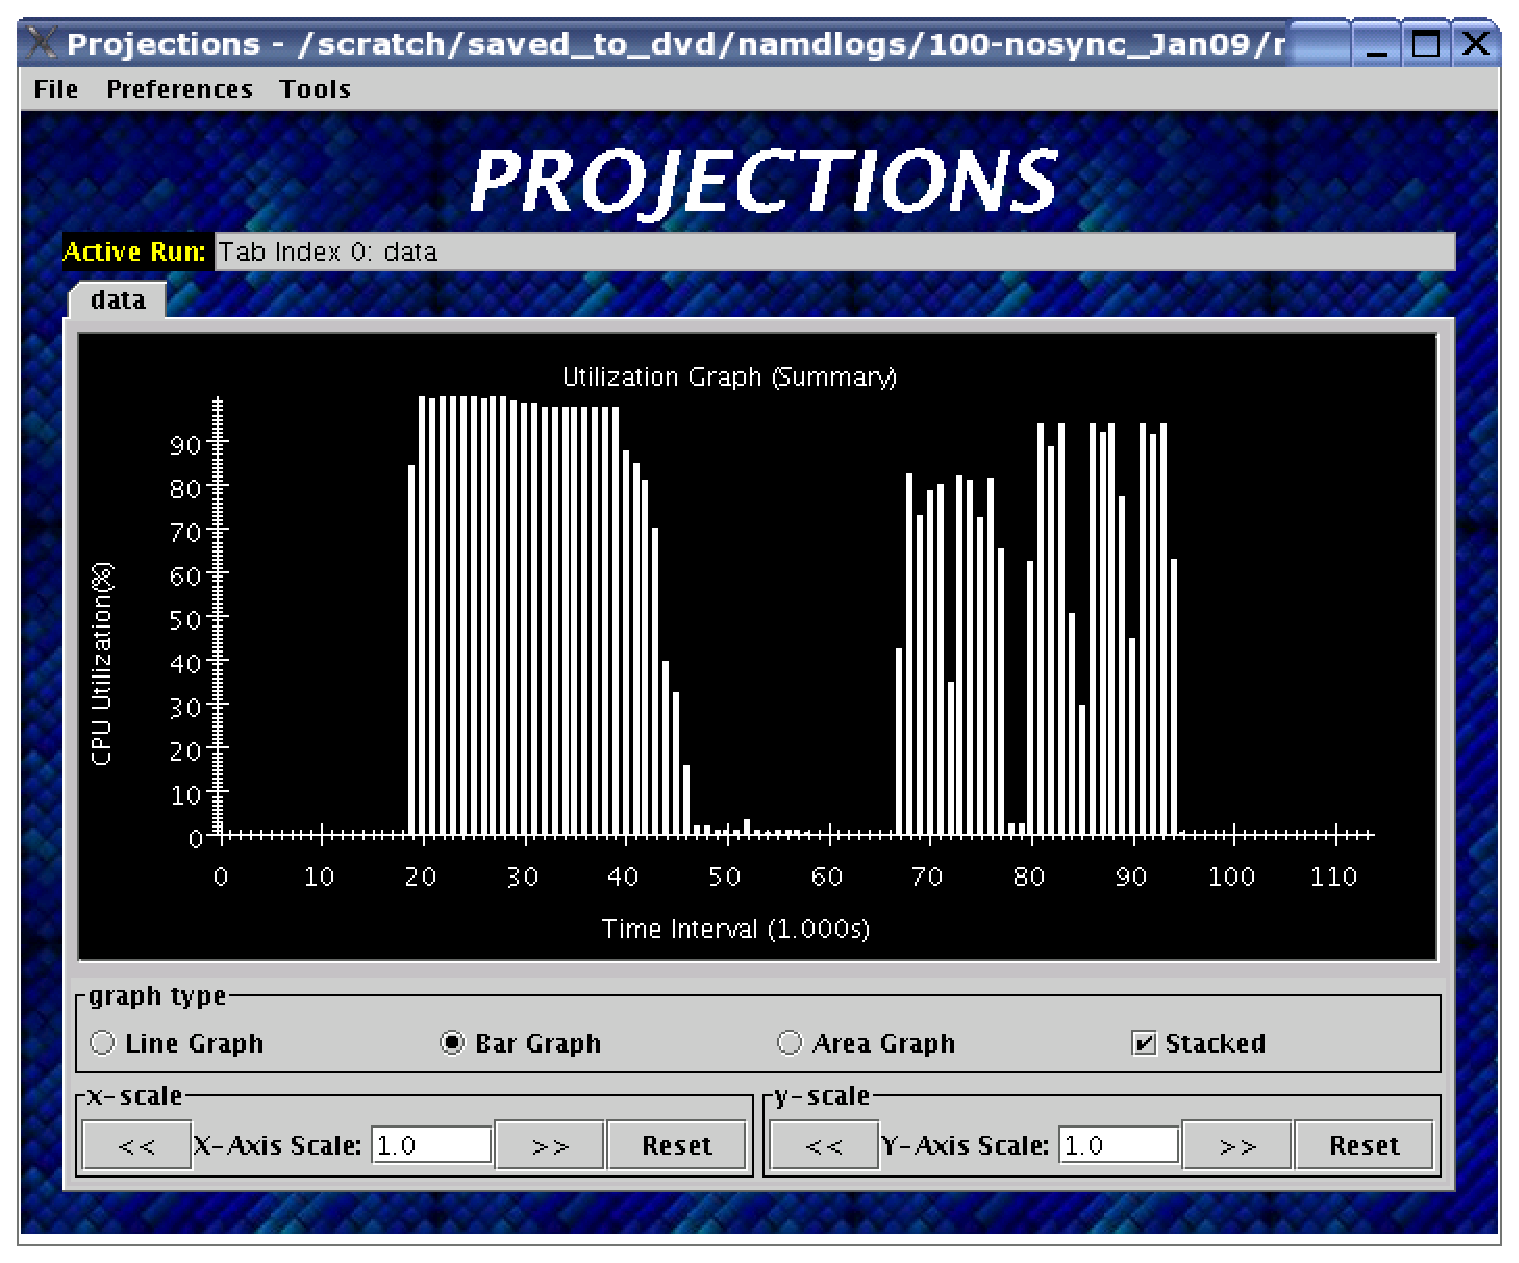
\includegraphics[width=4.0in]{fig/front-with-summary}
\caption{\projections{} main window}
\label{mainwindow}
\end{figure}

When \projections{} is started, it will display a main window as shown
in figure \ref{mainwindow}. If summary (.sum) files are available in
the set of data, a low-resolution utilization graph (Summary Display)
will be displayed as shown. If summary files are not available, or if
\projections{} was started without supplying the optional {\tt
NAME.sts} file, the main window will show a blank screen.

%{\bf Menu Options}

\begin{itemize}
\item
  {\bf File} contains 3 options. {\it Open File(s)} allows you to
  explicitly load a data set. This happens if you had not specified a
  {\tt NAME.sts} file in the command line when starting \projections{}
  or if you wish to explicitly load a new dataset. It brings up a
  dialog box that allows you to select the location of the dataset you
  wish to study. Navigate to the directory containing your data and
  select the .sts file.  Click on `Open'. If you have selected a valid
  file, \projections{} will load in some preliminary data from the
  files and then activate the rest of the options under the menu item
  {\bf Tools}. {\it Close current data} currently works the same way as 
  {\it Close all data}. They unload all current projections data so one can
  load in a new set of data. They will also deactivate the individual items
  provided in the {\bf Tools} menu option.
\item
  {\bf Preferences} generally allows you to set foreground or background
  colors and entry method color schemes. This is useful for configuring
  the color schemes of projections windows to be print-friendly.
\item
  {\bf Tools} lists the set of available tools for analysis of generated
  trace data. It will be described in great detail under section
  \ref{sec::available tools}.
\end{itemize}

%{\bf Summary Display}

The Summary Display loaded on the Main Window displays basic processor
utilization data (averaged across all processors) over time
intervals. This is provided by the data generated by the summary
tracemode. This view offers no special features over and above the
{\bf Standard Graph Display} described in section \ref{sec::misc}. 
Please refer the appropriate section on information for using
its available features.

%{\bf Summary Display Performance Issues}

There should not be any serious performance issues involved in the
loading of summary data on the main window.

\subsubsection{Available Tools}
\label{sec::available tools}

The following tools and views become available to you after a dataset
has been loaded (with the exception of Multirun Analysis) and may be
accessed via the menu item Tools:

\begin{itemize}
\item 
The {\bf Graphs} view is where you can analyze your data by breaking it
into any number of intervals and look at what goes on in each of those
intervals.
\item
The {\bf Timelines} view lets you look at what a specific processor is
doing at each moment of the program. It is the most detailed view of a
parallel application \projections{} offers (and correspondingly, the
most resource-hungry).
\item
The {\bf Usage Profile} view lets you see percentage-wise what entry
methods each processor spends its time on during a specified time range.
It is particularly useful for identifying load imbalance and the probable
offending entry method.
\item
The {\bf Communication} view is a general tool that presents
communication properties contributed by each entry point across the
processors.
\item
The {\bf Log File Viewer} provides a human-readable, verbose
interpretation of a log file's entries.
\item
The {\bf Histograms} view presents entry point or communication
histogram information (ie. the frequency of occurrence of events given
an activity property like time bin size or message size on the
x-axis).
\item
The {\bf Overview} view gives user an overview of the utilization of
all processors during the execution. It is an extremely useful initial
tool to begin your performance analysis efforts with as it provides an
overall picture of application performance while being very
light-weight at the same time.
\item
The {\bf Animation} view animates the processor usage over a specified
range of time and a specified interval size.
\item
The {\bf Time Profile Graph} view is a more detailed presentation of
the {\bf Graphs} utilization view in that it presents the time
contribution by each entry point across the desired time
interval. While the {\bf Graphs} view can show the same data, it is
unable to stack the entry points, which proves useful in some cases.
\end{itemize}

\subsubsection{Graphs}
\label{sec::graph view}

%{\bf Introduction}

The Graphs window (see figure \ref{graph}) is where you can analyze your data by breaking it
into any number of intervals and look at what goes on in each of those
intervals.

%{\bf Dialog Box}

When the Graph Window first appears, a dialog box will also appear. It
will ask for the following information (Please refer to
\ref{sec::misc} for information on special features you can
use involving the various fields)::

\begin{itemize}
\item
Processor(s): Choose which processor(s) you wish to visualize graph 
information for.
\item
Start Time : Choose the starting time of interest. A time-based field.
\item
End Time : Choose the ending time of interest. A time-based field.
\item
Interval Size : Determine the size of an interval. The number of intervals
will also be determined by this value (End Time - Start Time divided by
Interval Size). A time-based field.
\end{itemize}

Standard \projections{} dialog options and buttons are also available
(see \ref{sec::misc} for details).

The following menu items are available:

\begin{itemize}
\item
{\bf File} contains 2 options: {\it Print Graph} uses Java's built-in 
print manager feature to render the tool's displays (usually to a printer 
or a file depending on the platform on which Java is supported). Note that
the current implementation of the renderer does not behave in exactly the
same fashion as the screen renderer, so you should expect the output to look
somewhat different. {\it Close} simply closes the Graph window.
\item
{\bf Tools} contains 2 options: {\it Set Interval Size} reloads the dialog
box so you could select a new time range over which to view Graph data.
{\it Timeline} is currently not implemented. Its intended as a convenient
way to load Timeline data (see section \ref{sec::timeline view}) over the 
same parameters as the current Graph view.
\end{itemize}

%{\bf Tool Performance }

The amount of time to analyze your data depends on several factors,
including the number of processors, number of entries, and number of
intervals you have selected.  A progress meter will show the amount of
data loaded so far. The meter will not, however, report rendering
progress which is determined mainly by the number of intervals selected.
As a rule of thumb, limit the number of intervals to 1,000 or less.

\begin{figure}[hbt]
\center
%\epsfig{figure=fig/graph.eps,height=4.3in}
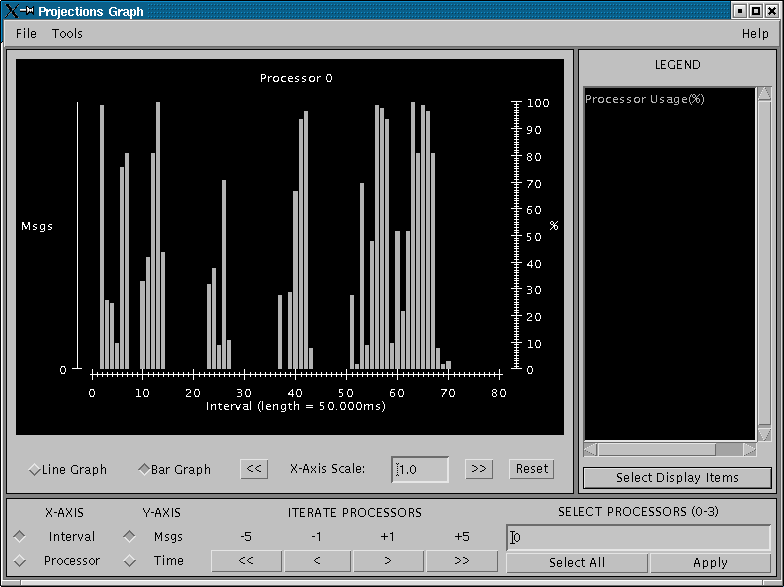
\includegraphics[width=4.3in]{fig/graph}
\caption{Graph tool}
\label{graph}
\end{figure}

%{\bf Tool Features }

The Graph Window has 3 components in its display:
\begin{enumerate}
\item[1)]
{\bf Display Panel} (located : top-left area)
   \begin{itemize}
   \item[-]
   Displays title, graph, and axes. To the left is a y-axis bar for
   detailed information involving the number of messages sent or time
   executed depending on the {\bf Control Panel} toggle selected (see 
   below). To the right is a y-axis bar for average processor-utilization 
   information. The x-axis may be based on time-interval or per-processor
   information depending on the appropriate {\bf Control Panel} toggle.
   \item[-]
   Allows you to toggle display between a line graph and a bar graph.
   \item[-]
   Allows you to scale the graph along the X-axis.  You can either
   enter a scale value $>=$ 1.0 in the text box, or you can use the
   $<<$ and $>>$ buttons to increment/decrement the scale by .25.
   Clicking on Reset sets the scale back to 1.0.  When the scale is
   greater than 1.0, a scrollbar will appear along the bottom of the
   graph to let you scroll back and forth.
   \end{itemize}
\item[2)]
{\bf Legend Panel} (located : top-right area)
   \begin{itemize}
   \item[-]
   Shows what information is currently being displayed on the graph and 
   what color represents that information.
   \item[-]
   Click on the `Select Display Items' button to bring up a window to
   add/remove items from the graph and to change the colors of the items:
      \begin{itemize}
      \item[*]
      The {\bf Select Display Items} window shows a list of items that you
      can display on the graph.  There are 3 main sections: System
      Usage, System Msgs, and User Entries. The System Usage and System
      Msgs are the same for all programs. The User Entries section
      has program-specific items in it.
      \item[*]
      Click on the checkbox next to an item to have it displayed on the
      graph.
      \item[*]
      Click on the colorbox next to an item to modify its color.
      \item[*]
      Click on `Select All' to choose all of the items
      \item[*]
      Click on `Clear All' to remove all of the items
      \item[*]
      Click on `Apply' to apply you choices/changes to the graph
      \item[*]
      Click on `Close' to exit
      \end{itemize}
   \end{itemize}
\item[3)]
{\bf Control Panel} (located : bottom area)
   \begin{itemize}
   \item[-]
   Allows you to toggle what is displayed on the X-axis.  You can either
   have the x-axis display the data by interval or by processor.
   \item[-]
   Allows you to toggle what is displayed on the Y-axis.  You can
   either have the y-axis display the data by the number of msgs sent
   or by the amount of time taken.
   \item[-]
   Allows you to change what data is being displayed by iterating
   through the selections.  If you have selected an x-axis type of
   `interval', that means you are looking at what goes on in each
   interval for a specific processor.  Clicking on the $<<, <, >, >>$
   buttons will change the processor you are looking at by either -5,
   -1, +1, or +5.  Conversely, if you have an x-axis of `processor',
   then the iterate buttons will change the value of the interval that
   you are looking at for each processor.
   \item[-]
   Allows you to indicate which intervals/processors you want to
   examine.  Instead of just looking at one processor or one interval,
   the box and buttons on the right side of this panel let you choose
   any number or processors/intervals to look at. This field behaves
   like a processor field. Please refer to section \ref{sec::misc} 
   for more information about the special features on using processor
   fields.

   Clicking on `Apply' updates the graph with your choices. Clicking
   on `Select All' chooses the entire processor range.  When you
   select more than one processor's worth of data to display, the
   graph will show the desired information summed across all selected
   processors. The exception to this is processor utilization data
   which is always displayed as data averaged across all selected
   processors.
   \end{itemize}
\end{enumerate}

\subsubsection{Timelines}
\label{sec::timeline view}

%{\bf Introduction}

The Timeline window (see figure \ref{timeline}) lets you look at what
a specific processor is doing at each moment of the program.

\begin{figure}[htb]
\center
%\epsfig{figure=fig/timeline.eps,height=3.8in}
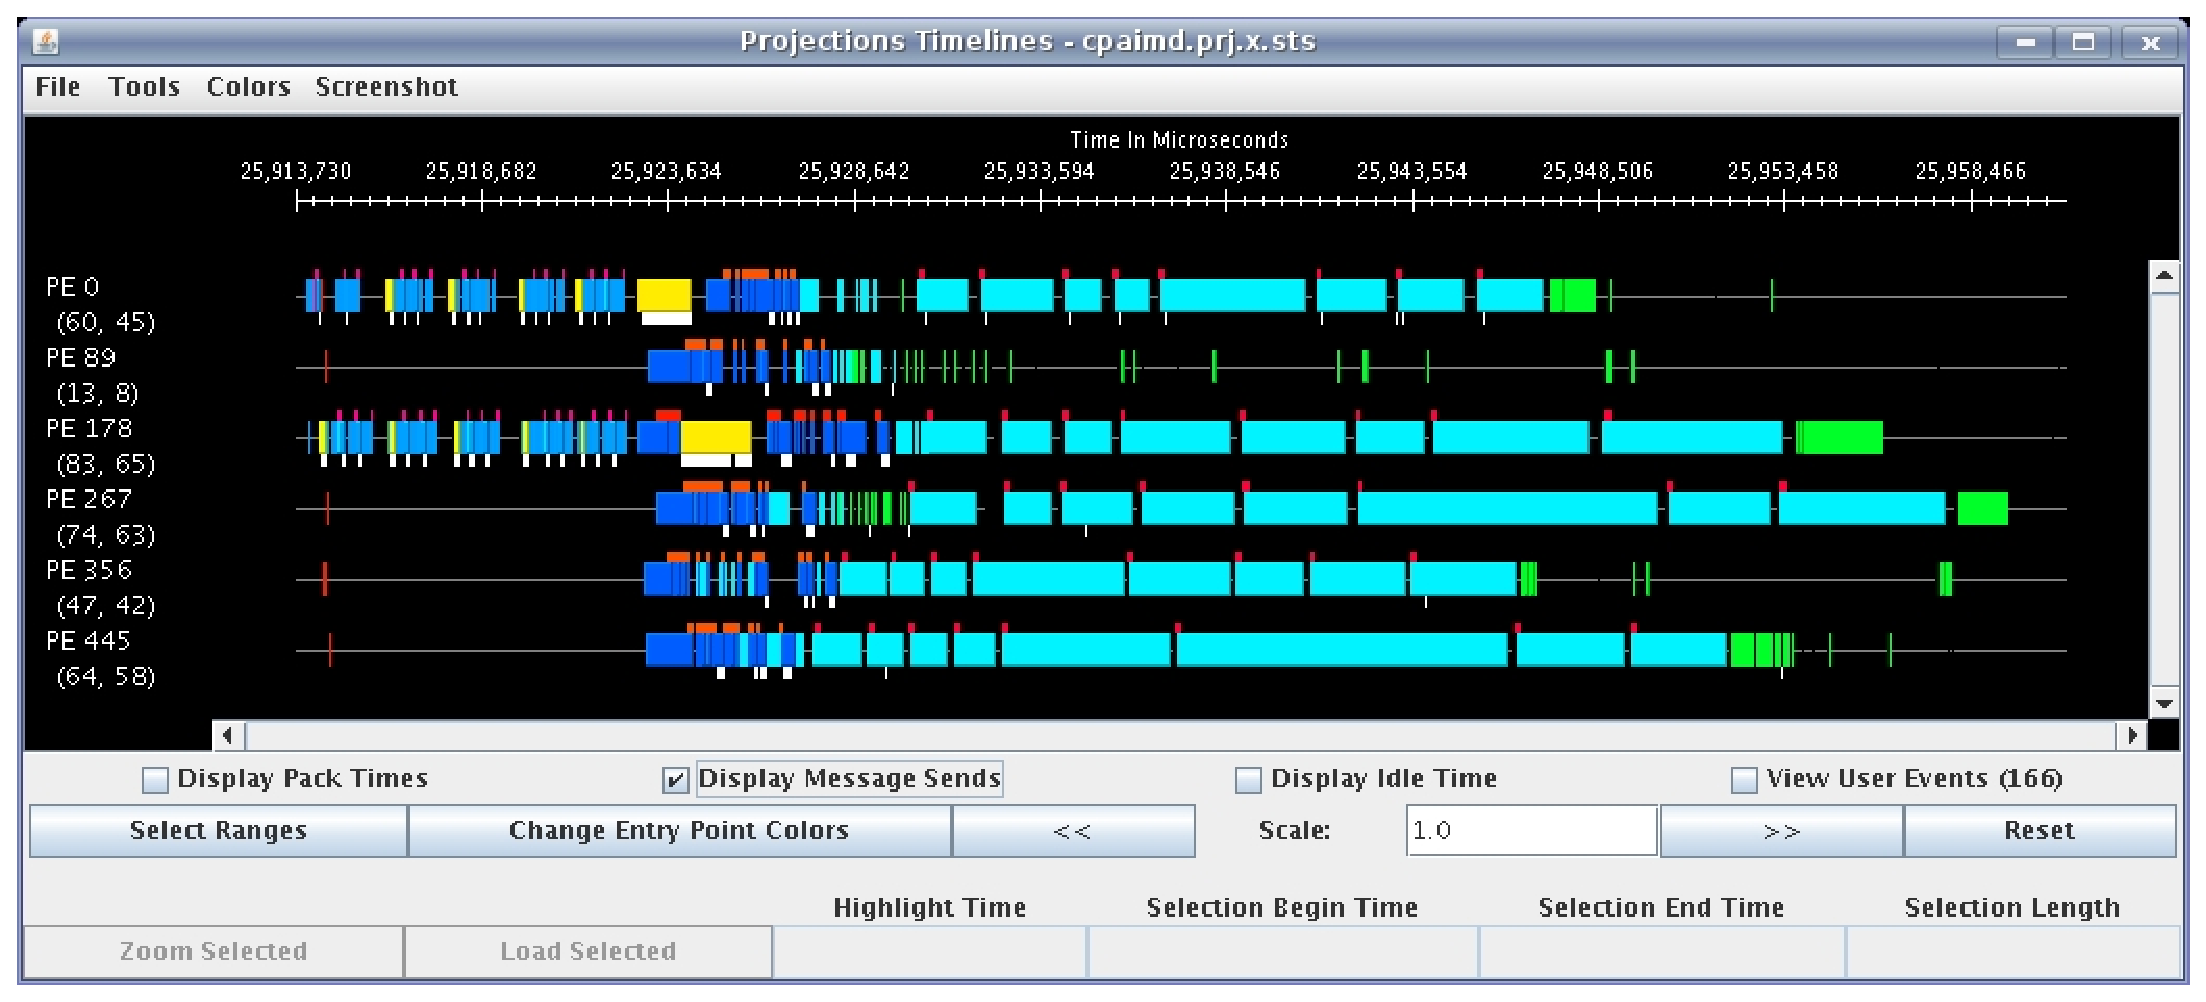
\includegraphics[width=3.8in]{fig/timeline}
\caption{Timeline module}
\label{timeline}
\end{figure}

%{\bf Dialog Box}

When the Timeline window first appears, a dialog box appears along
with it. The box asks for the following information (Please refer to
\ref{sec::misc} for information on special features you can
use involving the various fields):

\begin{itemize}
\item
Processor(s): Choose which processor(s) you want to see a timeline
for.
\item
Start Time  : Choose what time you want your timeline to start at.
A time-based field.
\item
End Time    : Choose what time you want your timeline to end at. A time-based
field.
\end{itemize}

Standard \projections{} dialog options and buttons are also available
(see \ref{sec::misc} for details).

{\bf Special Note} : {\it The current timeline main display fails to
size itself properly when first loaded. This gives the impression that
no timeline data was loaded as only the control panel shows up,
confusing most users. All you have to make the main display show up is
to resize the window after loading. This can be done manually or by
using the window's maximize feature, available on most Java
platforms. We recommend the latter.}

%Instead of entering a BeginTime, you can have the dialog box choose a
%BeginTime for you based on the occurrence of a specific entry.  To do
%this, you go to the bottom portion of the dialog box and select an
%entry to find an occurrence of.  Then, you choose the processor you
%want to find an occurrence on, and which occurrence you want to find
%(N). Click on 'Search for Begin Time'.  The dialog box will display a
%message telling you if your occurrence was found and when it was
%found. If valid, the time is automatically entered as the begin time.

%When you are satisifed with your time and processor ranges, click on
%'OK'.  \projections{} will then get the Timeline data for you.  The
%time for this step depends on the number of items in your time range
%and the number of processors you have chosen.

%{\bf Tool Features}

The following menu options are available:

\begin{itemize}
\item {\bf File} contains 2 options: {\it Print Timeline} uses Java's
built-in print manager and allows you to render the timeline's display
onto a physical printer or file. Currently, the code used to render
the timeline display for printing differs significantly from that used
to render the display to screen, so please expect differences. 
{\it Close} simply closes the Timeline Window.
\item {\bf Tools} contains 1 option: {\it Modify Ranges} reloads the 
dialog box and allows you to select new processor or time duration
parameters.
\item {\bf Colors} contains 4 options: {\it Change Colors} functions in
a manner similar to the button of the same name described under control 
panel information below. {\it Save Colors} allows you to save the current
color set to a file named ``color.map'' into the same directory where your
data logs are stored. Note that the directory must have write permissions
for you before this can work. We are currently working on a more flexible
scheme for storing saved color sets. {\it Restore Colors} allows you to
load any previously saved color sets described above. {\it Default Colors}
resets the current color set to the default set that \projections{} assigns
without user intervention.
\end{itemize}

The Timeline Window consists of two parts:
\begin{enumerate}
\item[1)]
{\bf Display Panel} (located: top area)

This is where the timelines are displayed and is the largest portion
of the window.  The time axes are displayed at the top and the bottom
of the panel, and the units are microseconds.  The left side of the
panel shows the processor labels.  Underneath each processor label is
a percentage telling you what amount of the total time in your
timeline was actually spent working on this program.

The timeline itself consists of colored bars for each work item.
Placing the cursor over one of these bars will bring up a pop-up
window telling you the name of that item, the begin time, the end
time, and the total time.  It will also tell you what amount of time
was spent packing, how many messages were created during this work
item, and which processor created this item. 

User events are also displayed as thin lines or bars above ordinary
event bars in the display area.

Display Panel features include:
   \begin{itemize}
   \item[-] 
   Detailed Information Pop-up - If you left-click on an item, a
   window will appear telling you similar information to the pop-up
   window.  This window will also list all of the messages created
   during this work item, and it will tell you what time they were
   sent at and to which entry.
   \item[-]
   Message Source Lines - If you right-click on an item, a white line
   will be drawn from the beginning of that item to the source of the
   message send that created the item. This line can only be drawn if
   the source lies within the loaded time range. Additionally, if the
   processor on which the source lies is not loaded, \projections{}
   will automatically load it into the timeline.
   \end{itemize}

\item[2)]
{\bf Control Panel} (located: bottom area)

Checkboxes:
   \begin{itemize}
   \item[-]
   Display Pack Times - Lets you toggle display of Time spent packing
   \item[-] 
   Display Message Creations - Lets you toggle display of message
   creations. These are represented by little vertical lines at the
   time a message was created.
   \item[-]
   Display Idle Time - Lets you toggle display of idle time.
   \item[-] 
   View User Event - Checking this box will bring up a new
   window showing the string description, begin time, end time and
   duration of all user events on each processor. You can access
   information on user events on different processors by accessing the
   numbered tabs near the top of the display.

   \begin{figure}[htb]
   \center
%\epsfig{figure=fig/userevent.eps,height=1.5in}
   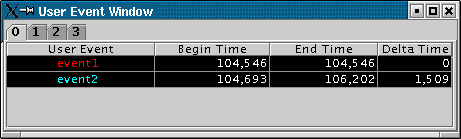
\includegraphics[height=1.5in]{fig/userevent}
   \caption{User Event Window}
   \label{userevent}
   \end{figure}

   \end{itemize}

Buttons:
   \begin{itemize}
   \item[-]
   Select Ranges - Brings up the initial dialog box.
   \item[-]
   Change Colors - Lets you change colors for the work items.
   \item[-]
   Scale - Enter a scale $>=$ 1.0 in the box, or click on the $<<$ and
   $>>$ buttons to adjust the scale by 0.25 increments.  Click on
   Reset to set the scale back to 1.0
   \end{itemize}
\end{enumerate}

An additional feature of timeline is a quick interface to zoom into an
area of interest. To determine the exact time of any event on the
timeline, move your mouse along either the top or bottom axis and a
white vertical highlight line will show where your cursor is along the
timeline. The ``Highlight Time'' box on the bottom of the Timeline
window will show the exact time based on the location of your cursor.

To select an area, click on the axis to define the start of the area
and drag the mouse to the end of the area to be defined.  Two yellow
vertical lines will bracket the area of interest.  The exact times of
the selected area will be shown in the ``Selection Start Time'' text
area and the ``Selection End Time'' text area.  The difference between
these times is shown in ms in the ``Selected Length'' text area.  Thus,
this feature can be used to measure the time between two events of
interest across processors, and is an easy way to measure the time of
an entry point.

To then zoom into the selected area via this interface, click on
either the ``Zoom Selected'' or the ``Load Selected'' buttons.  The
difference between these two buttons is that the "Load Selected" zooms
into the selected area and discards any events that are outside the
time range.  This is more efficient than ``Zoom Selected'' as the
latter draws all the events on a virtual canvas and then zooms into
the canvas. The disadvantage of using ``Load Selected'' is that it
becomes impossible to zoom back out without having to re-specify the
time range via the ``Select Ranges'' button.

Performance-wise, this is the most memory-intensive part of the
visualization tool. Users should expect long load and/or display
times. This is dependent on the number of event objects to be
displayed (multiplied by the number of processors to be
displayed). The selected time range is a loose approximation of this
but the user should be aware of how event-intensive the application is
over the desired time-period before proceeding to use this view. If
\projections{} becomes stalled as a result of an attempt to load too
much data, kill the visualization tool and restart the analysis with a
smaller time/processor range. We expect to add features to alleviate
this problem in future releases.

\subsubsection{Usage Profile}

The Usage Profile window (see figure \ref{usage profile}) lets you see
percentage-wise what each processor spends its time on during a
specified period.

When the window first comes up, a dialog box appears asking for the
processor(s) you want to look at as well as the time range you want to
look at.  This dialog functions in exactly the same way as for the Timeline
tool (see section \ref{sec::timeline view}).

\begin{figure}[htb]
\center
%\epsfig{figure=fig/usageprofile.eps,height=4in}
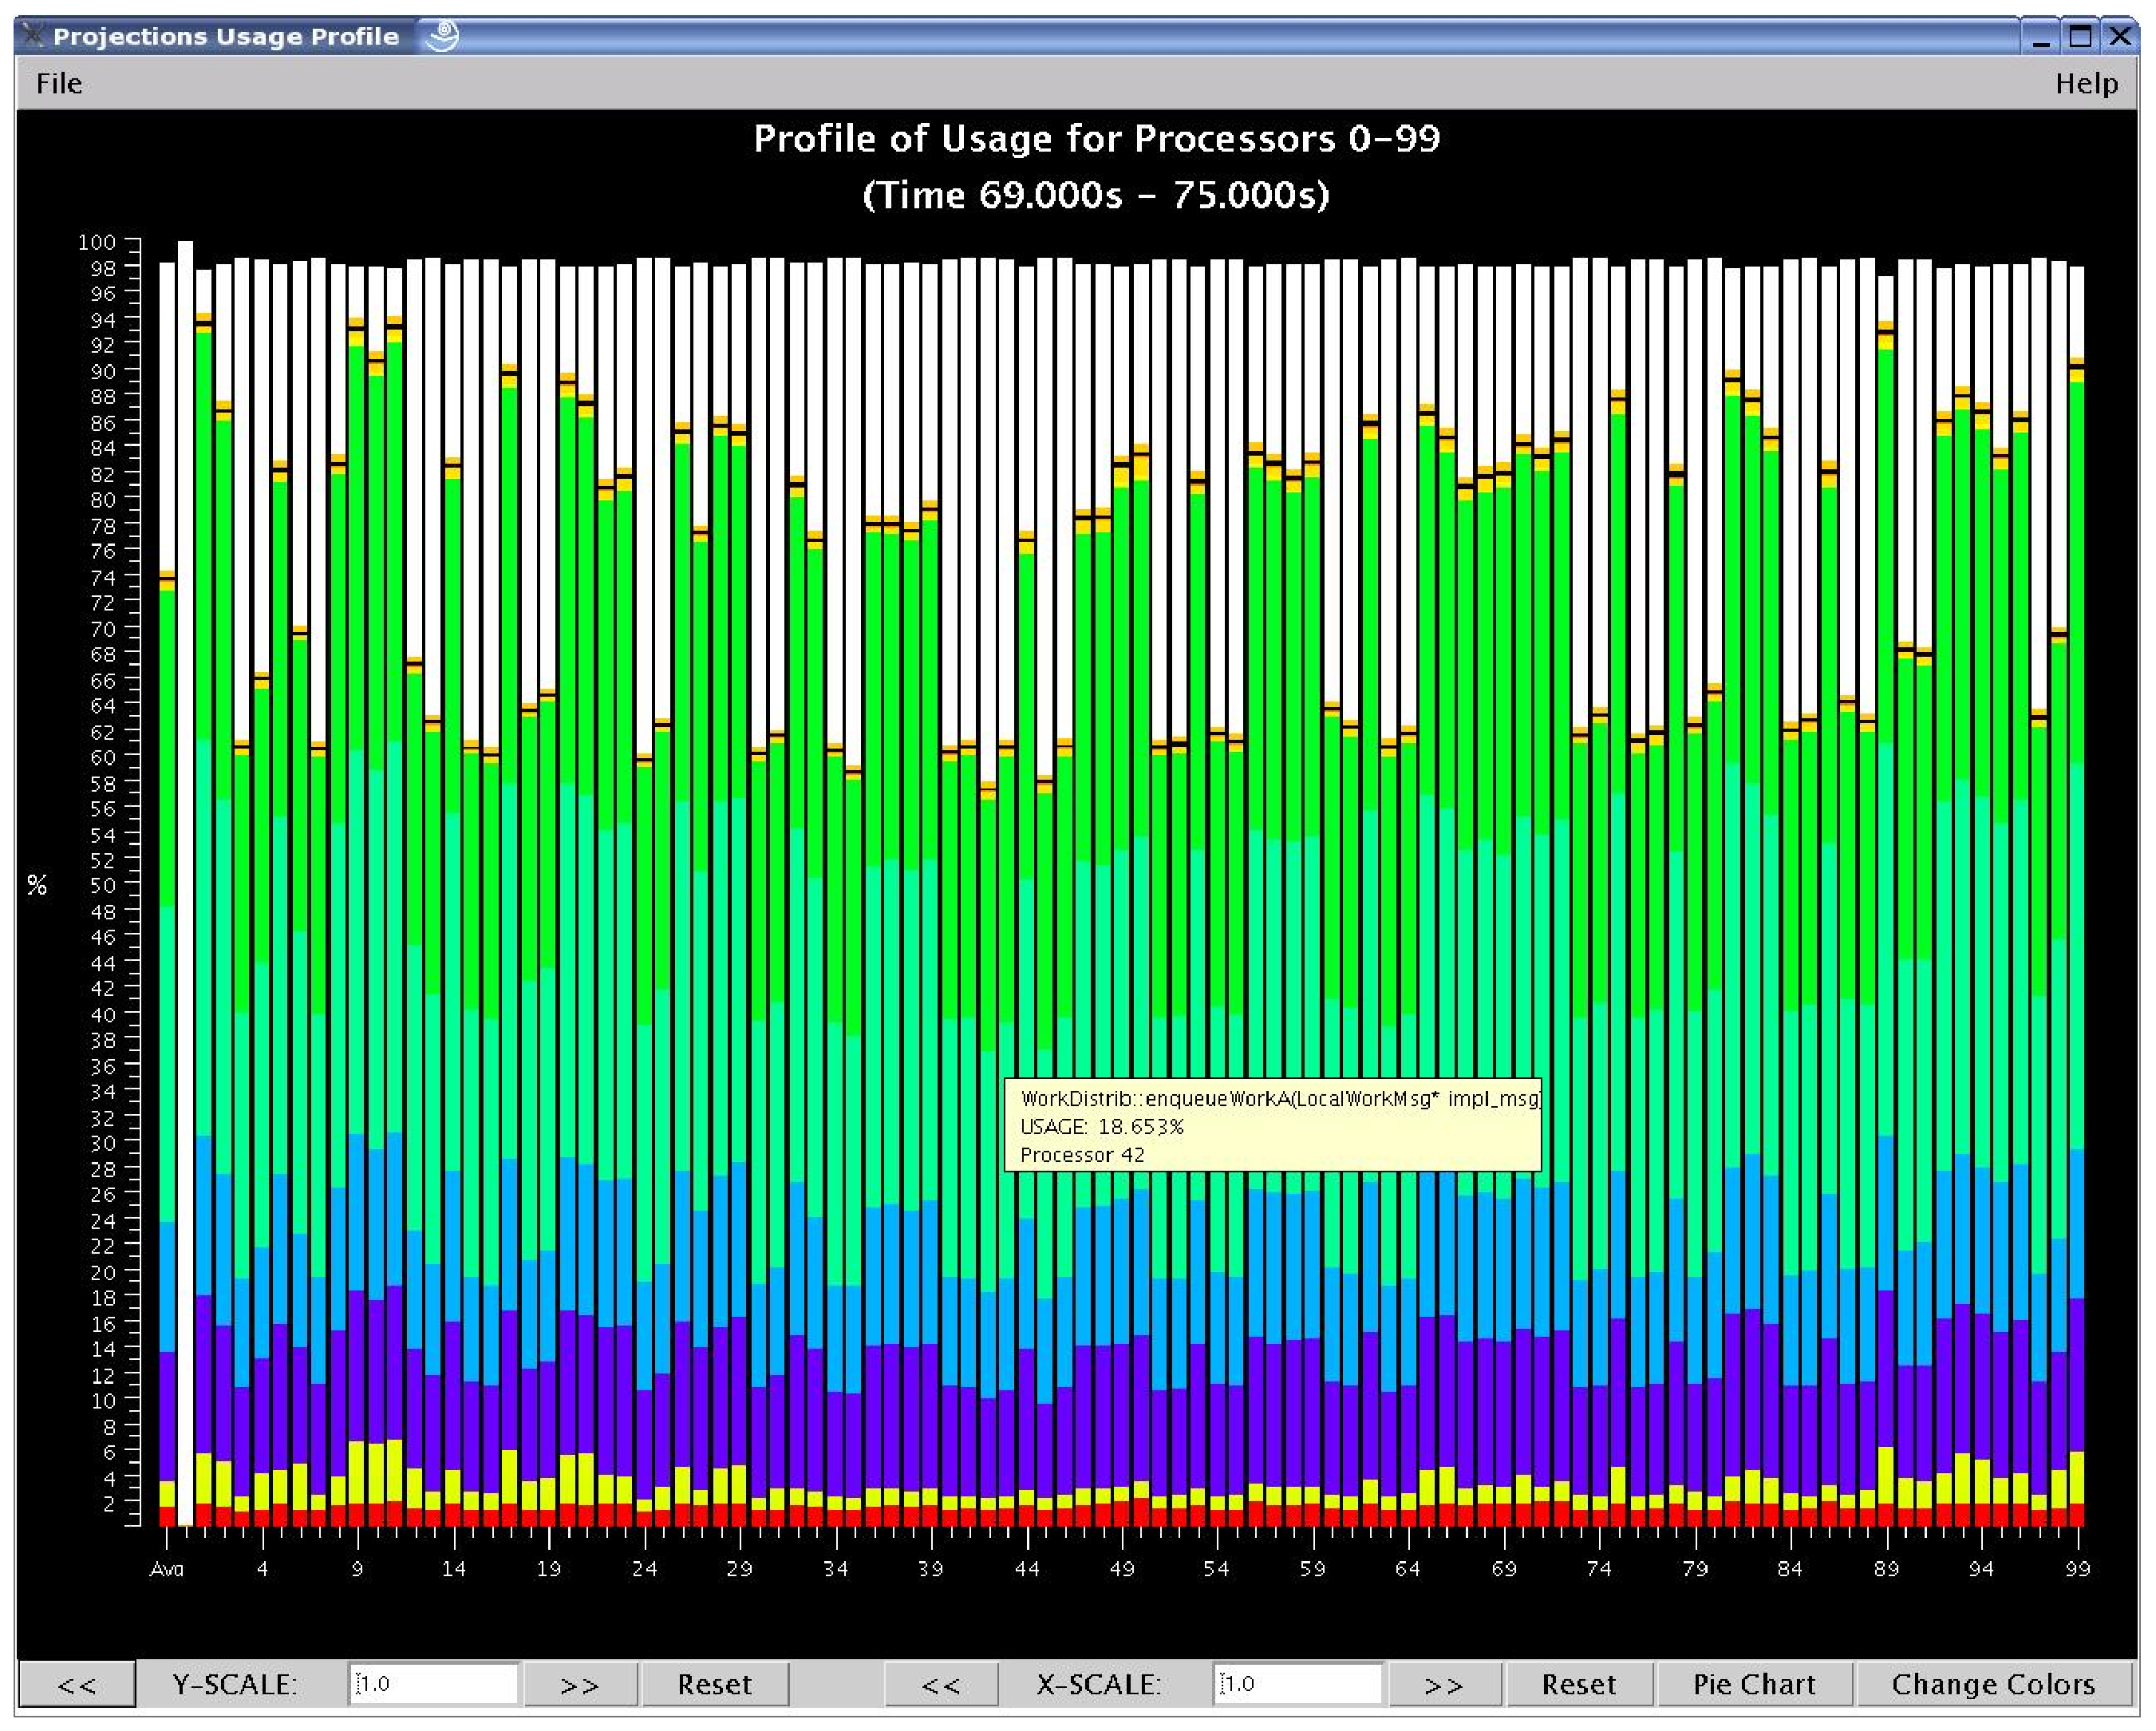
\includegraphics[width=4.0in]{fig/usageprofile}
\caption{Usage Profile}
\label{usage profile}
\end{figure}

The following menu options are available in this view:

\begin{itemize}
\item {\bf File} has 2 options: {\it Select Processors} reloads the dialog
box for the view and allows you to select a new processor and time range
for this view. {\it Print Profile} currently does nothing. This will be
addressed in a later release of \projections{}.
\end{itemize}

The following components are supported in this view:

\begin{itemize}
\item[1)] 
{\bf Main Display} (located: top area) 
The left axis of the display shows a scale from 0\% to 100\%.  The
main part of the display shows the statistics.  Each processor is
represented by a vertical bar with the leftmost bar representing the
statistics averaged across all processors. The bottom of the bar
always shows the time spent in each entry method (distinguished by the
entry method's assigned color) . Above that is always reported the
message pack time (in black), message unpack time (in orange) and idle
time (in white). Above this, if the information exists, are colored
bars representing communication CPU overheads contributed by each
entry method (again, distinguished by the same set of colors
representing entry methods). Finally the black area on top represents
time overheads that the charm++ runtime cannot account for.

If you mouse-over a portion of the bar (with the exception of the
black area on top), a pop-up window will appear telling you the name
of the item, what percent of the usage it has, and the processor it is
on.

\item[2)]
{\bf Control Panel} (located: bottom area)
The panellets you adjust the scales in both the X and Y directions.
The X direction is useful if you are looking at a large number of
processors. The Y direction is useful if there are small-percentage
items for a processor. The ``Reset'' button allows you to reset the 
X and Y scales.

The ``Pie Chart'' button generates a pie chart representation (see
figure \ref{piechart}) of the same information using averaged
statistics but without idle time and communication CPU overheads.

\begin{figure}[htb]
\center
%\epsfig{figure=fig/piechart.eps,height=1in}
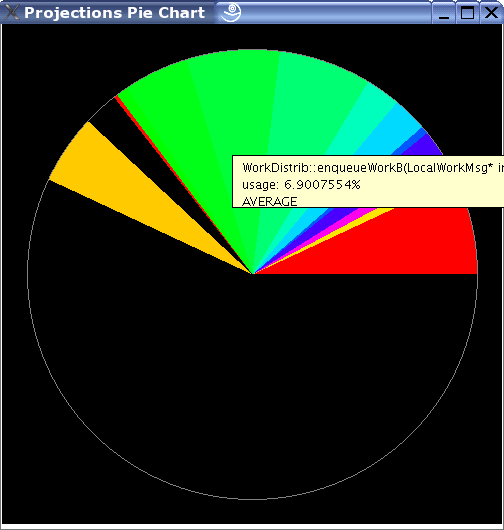
\includegraphics[width=1.8in]{fig/piechart}
\caption{Pie Chart representation of average usage}
\label{piechart}
\end{figure}

The ``Change Colors'' button lists all entry methods displayed on the
main display and their assigned colors. It allows you to change those
assigned colors to aid in highlighting entry methods.

The resource consumption of this view is moderate. Load times and
visualization times should be relatively fast, but dismissing the tool
may result in a very slight delay while \projections{} reclaims memory
through Java's garbage collection system.

\end{itemize}

\subsubsection{Communication}

The communication tool (see figure \ref{communication}) visualizes
communication properties on each processor over a user-specified time
range.

The dialog box of the tool allows you to specify the time period
within which to load communication characteristics information. This
dialog box is exactly the same as that of the Timeline tool (see
section \ref{sec::timeline view}).

The main component employs the standard capabilities provided by
\projections{}' standard graph (see \ref{sec::misc}).

The control panel allows you to switch between the following
communication characteristics:

\begin{itemize}
\item[-] Number of Messages Sent by entry methods (initial default view);
\item[-] Number of Bytes Sent by entry methods;
\item[-] Number of Messages Received by entry methods;
\item[-] Number of Bytes Received by entry methods;
\item[-] Number of Messages Sent externally (physically) by entry methods;
\item[-] Number of Bytes Sent externally (physically) by entry methods;
\item[-] and Number of hops messages travelled before being received
by an entry methods (available only on trace logs generated on the
Bluegene machine).
\end{itemize}

\begin{figure}[htb]
\center
%\epsfig{figure=fig/commhistogram.eps,height=4in}
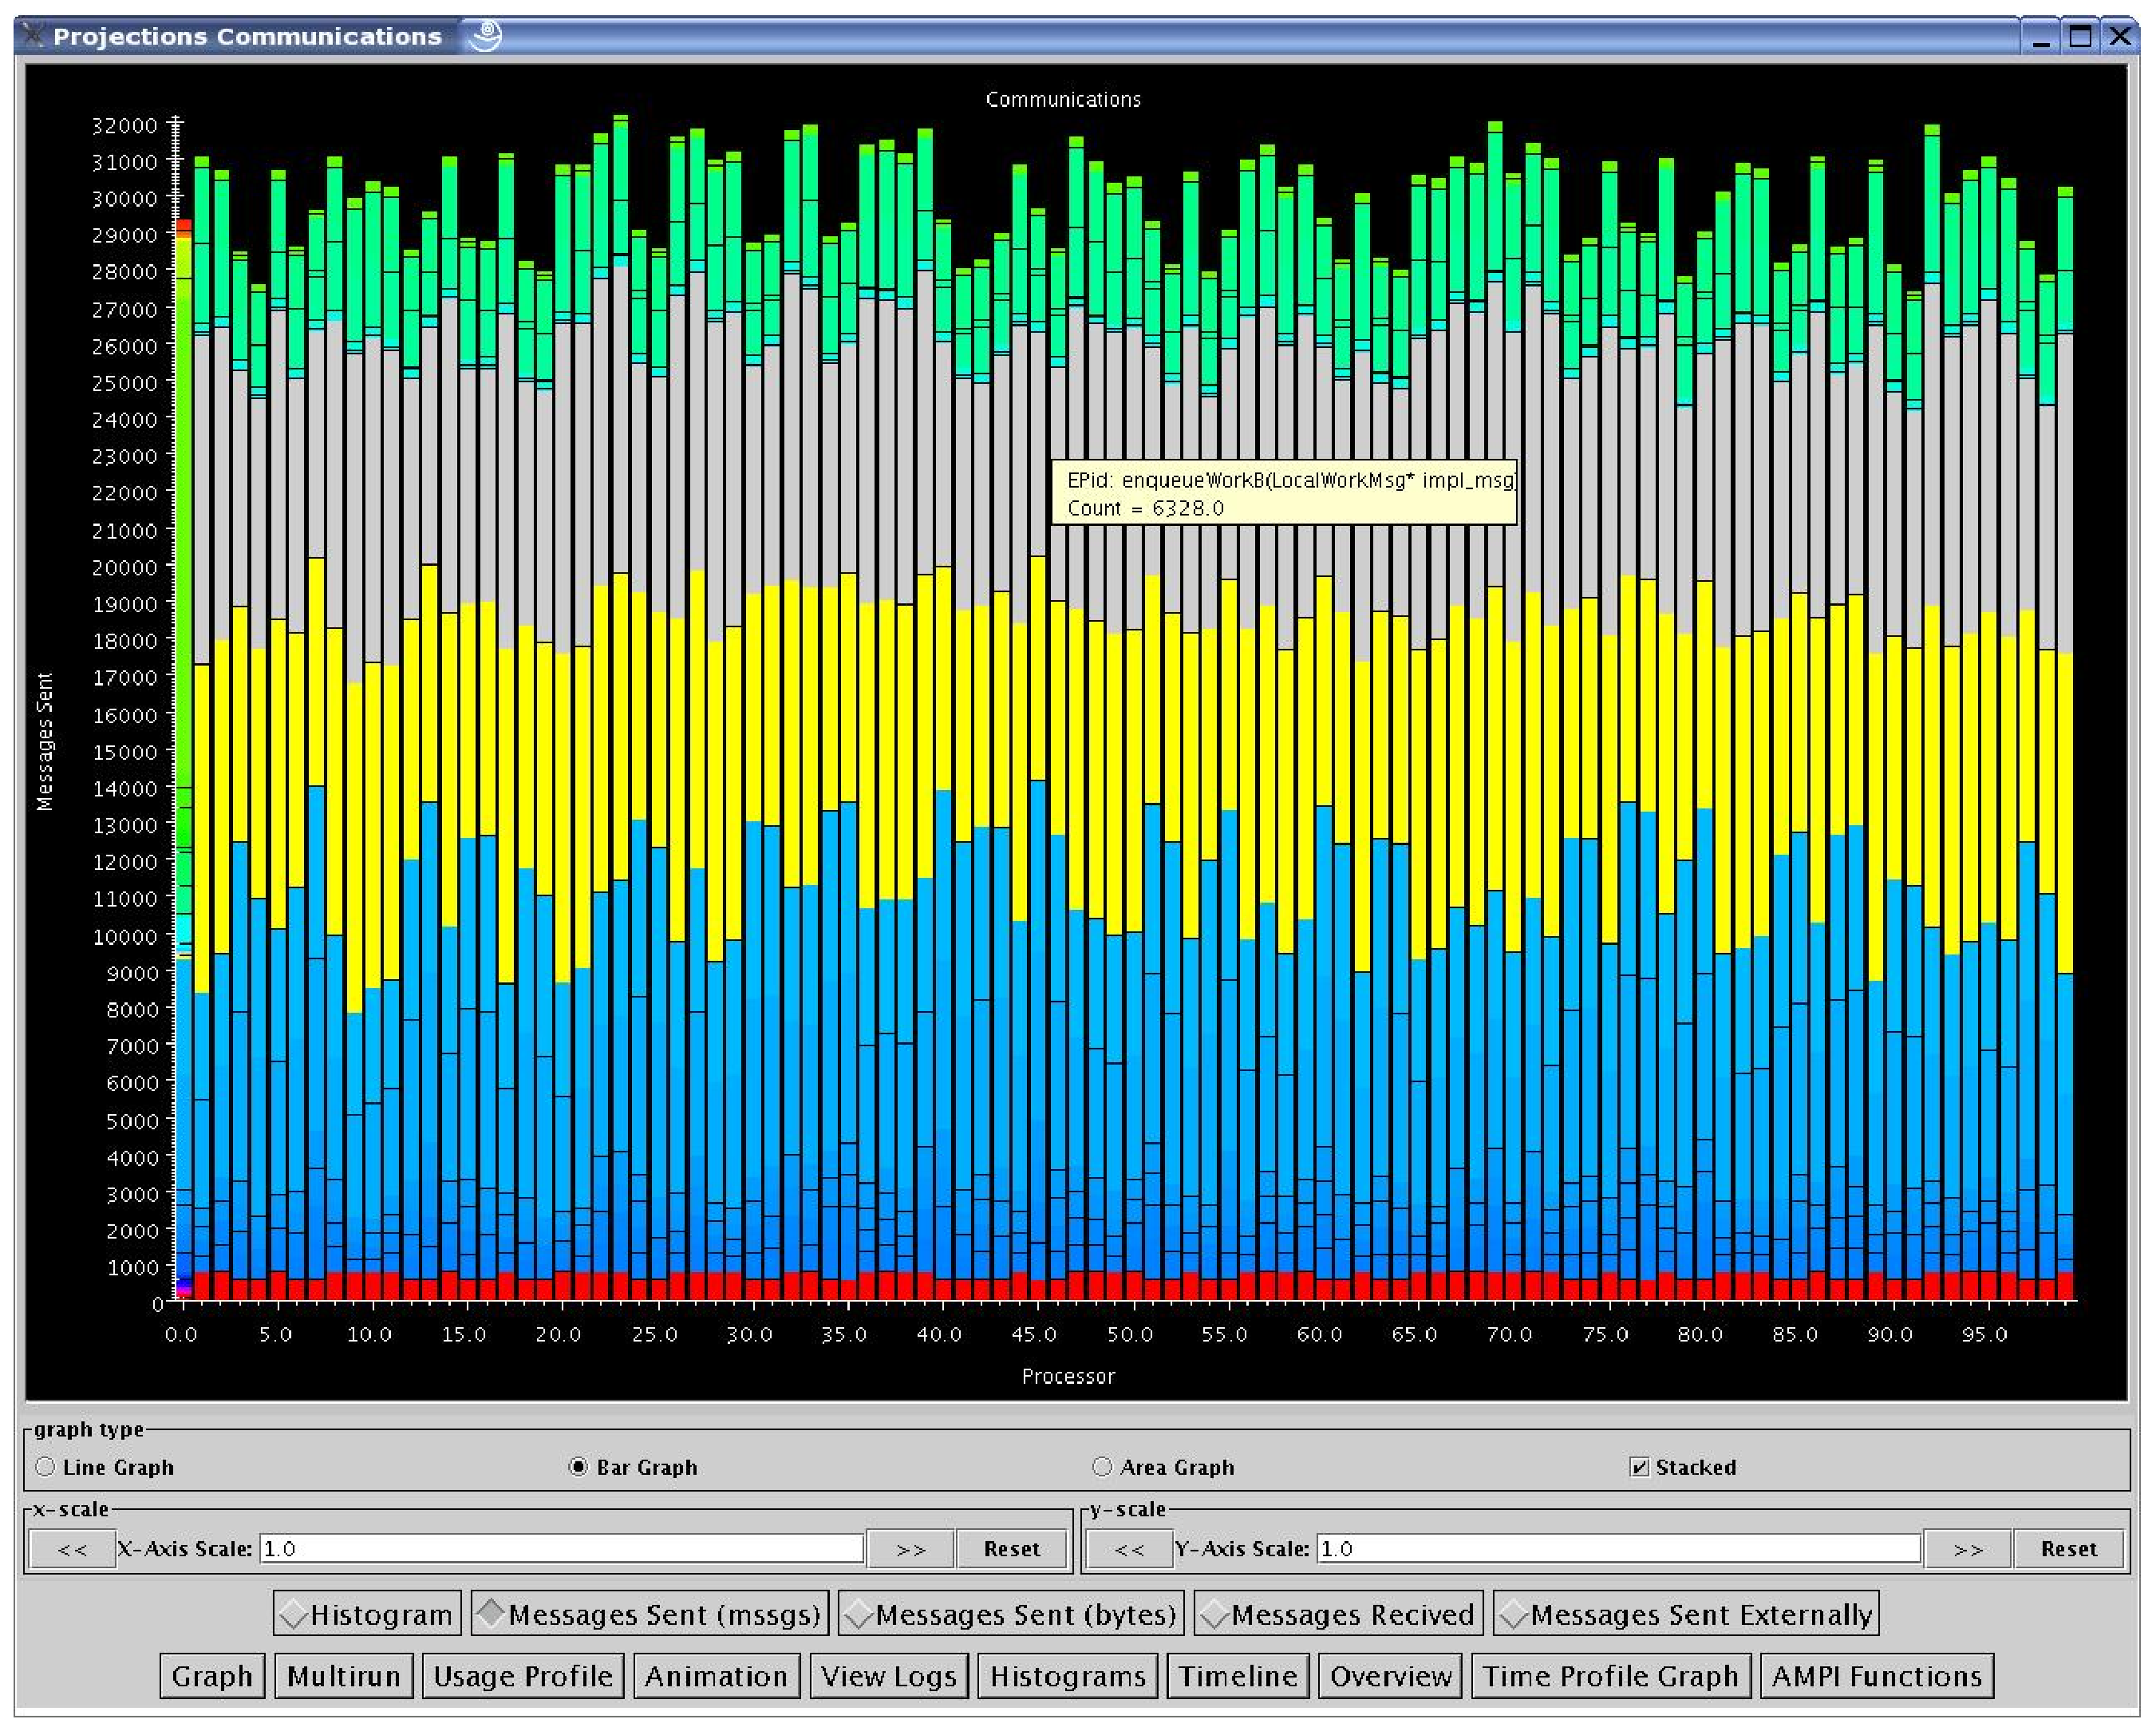
\includegraphics[width=4.0in]{fig/commhistogram}
\caption{Communication View}
\label{communication}
\end{figure}

This view has no known problems loading any range or volume of data.

\subsubsection{View Log Files}

This window (see figure \ref{viewlog}) lets you see a translation of a
log file from a bunch of numbers to a verbose version.  A dialog box
asks which processor you want to look at.  After choosing and pressing
OK, the translated version appears. Note that this is {\it not} a
standard processor field. This tool will only load {\it exactly} one
processor's data.

\begin{figure}[htb]
\center
%\epsfig{figure=fig/viewlog.eps,height=4in}
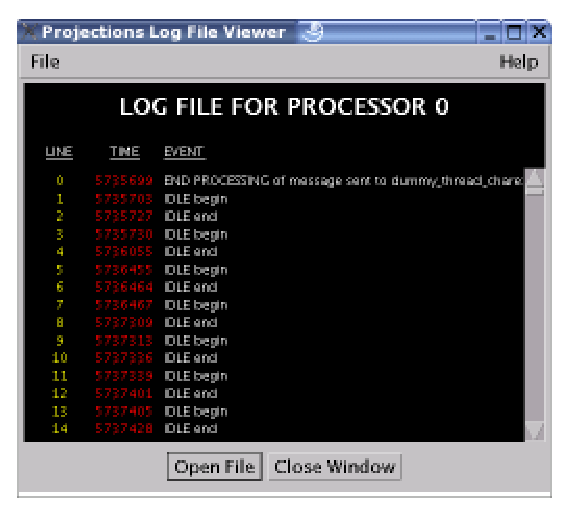
\includegraphics[width=2.5in]{fig/viewlog}
\caption{Log File View}
\label{viewlog}
\end{figure}

Each line has:
\begin{itemize}
\item[-] a line number (starting at 0)
\item[-] the time the event occurred at
\item[-] a description of what happened.
\end{itemize}

This tool has the following menu options:

\begin{itemize}
\item {\bf File} has 2 options: {\it Open File} reloads the dialog box
and allows the user to select a new processor's data to be loaded.
{\it Close} closes the current window.
\item {\bf Help} has 2 options: {\it Index} currently does not do anything.
This will be addressed in a later release of \projections{}. {\it About}
currently does not do anything. This will also be addressed in a later
release of \projections{}.
\end{itemize}

The tool has 2 buttons. ``Open File'' reloads the dialog box (described 
above) and allows the user to select a new processor's data to be loaded.
``Close Window'' closes the current window.

\subsubsection{Histograms}

This module (see figure \ref{histogram}) allows you to examine the
performance property distribution of all your entry points (EP). It
gives a histogram of different number of EP's that have the following
properties falling in different property bins:

The dialog box for this view asks the following information from the
user. (Please refer to \ref{sec::misc} for information on special
features you can use involving the various fields):

\begin{itemize}
\item
Processor(s): Choose which processor(s) you wish to visualize histogram
information for.
\item
Start Time: Choose the starting time of interest. A time-based field.
\item
End Time: Choose the ending time of interest. A time-based field.
\item
Number of Bins: Select the number of property bins to fit frequency data
under. A simple numeric field.
\item
Size of Bin: Determine (in units - microseconds or bytes) how large each
bin should be. A simple numeric field.
\item
Starting Bin Size: Determine (in units - microseconds or bytes) how
far to offset the data. This is useful for ignoring data that is too
small to be considered significant, but could overwhelm other data
because of the sheer numbers of occurrences. A simple numeric field.
\end{itemize}

The dialog box reports the selection of bins as specified by the user
by displaying the minimum bin size (in units - microseconds or bytes)
to the maximum bin size. ``units'' refer to microseconds for time-based
histograms or bytes for histograms representing message sizes.

Standard graph features can be employed for the main display of this
view (see section \ref{sec::misc}). 

The following menu items are available in this tool:

\begin{itemize}
\item {\bf File} offers 3 options: {\it Select Entry Points} currently
does nothing. It is intended to behave similarly to the button ``Select
Entries'' described below. This will be fixed in a later release of
\projections{}. {\it Set Range} reloads the dialog box and allows the
user to load data based on new parameters. {\it Close} closes the current
tool window.
\item {\bf View} provides 1 option: {\it Show Longest EPs} currently
does nothing. It is intended to behave similarly to the button 
``Out-of-Range EPs'' and will be fixed in a later release of \projections{}.
\end{itemize}

The following options are available in the control panel in the form
of toggle buttons:

\begin{itemize}
\item[-] Entry method execution time (How long did that entry method ran 
for?)
\item[-] Entry method creation message size (How large was the message
that caused the entry method's execution?)
\end{itemize}

\begin{figure}[htb]
\center
%\epsfig{figure=fig/histogram.eps,height=4in}
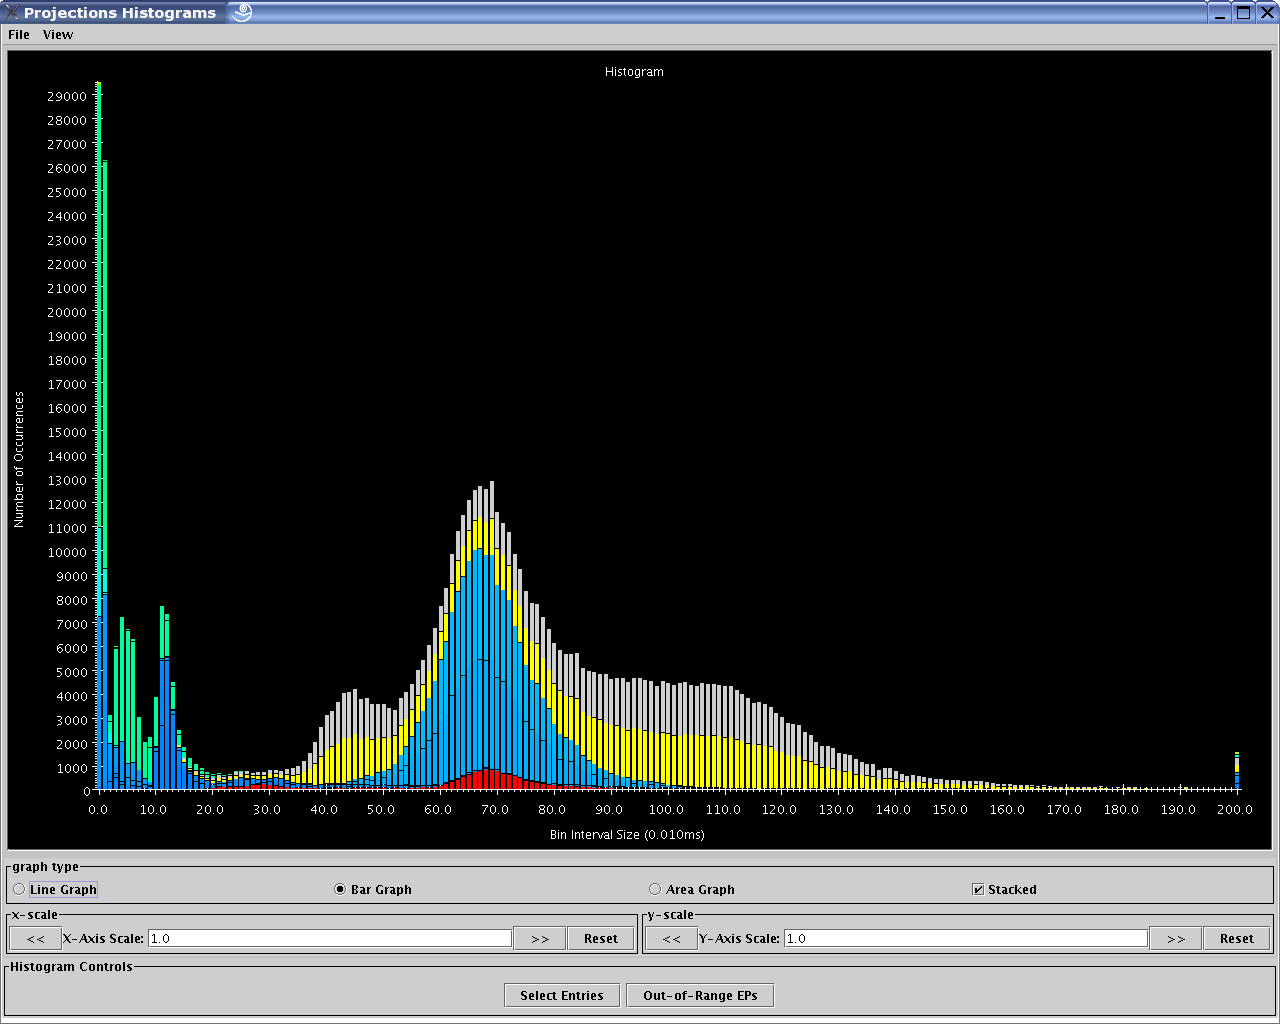
\includegraphics[width=4.0in]{fig/histogram}
\caption{Histogram view}
\label{histogram}
\end{figure}

The use of the tool is somewhat counterintuitive. The dialog box is
created immediately and when the tool window is created, it is
defaulted to a time-based histogram. You may change this histogram to
a message-size-based histogram by selecting the ``Message Size'' radio
button which would then update the graph using the same parameters
provided in the dialog box. This issue will be fixed in upcoming
editions of \projections{}.

The following features are, as of this writing, not implemented. They
will be ready in a later release of \projections{}.

The ``Select Entries'' button is intended to bring up a color
selection and filtering window that allows you to filter away entry
methods from the count. This offers more control over the analysis
(e.g. when you already know EP 5 takes 20-30ms and you want to know if
there are other entry points also takes 20-30ms).

The ``Out-of-Range EPs'' button is intended to bring up a table
detailing all the entry methods that fall into the overflow (last)
bin. This list will, by default, be listed in descending order of time
taken by the entry methods.

The performance of this view is affected by the number of bins the
user wishes to analyze. We recommend the user limits the analysis to
1,000 bins or less.

\subsubsection{Overview}

Overview (see figure \ref{overview}) gives users an overview of the
utilization of all processors during the execution over a
user-specified time range.

The dialog box of the tool allows you to specify the time period
within which to load overview information. This dialog box is exactly
the same as that of the Timeline tool (see section \ref{sec::timeline
view}).

\begin{figure}[htb]
\center
%\epsfig{figure=fig/overview.eps,height=4in}
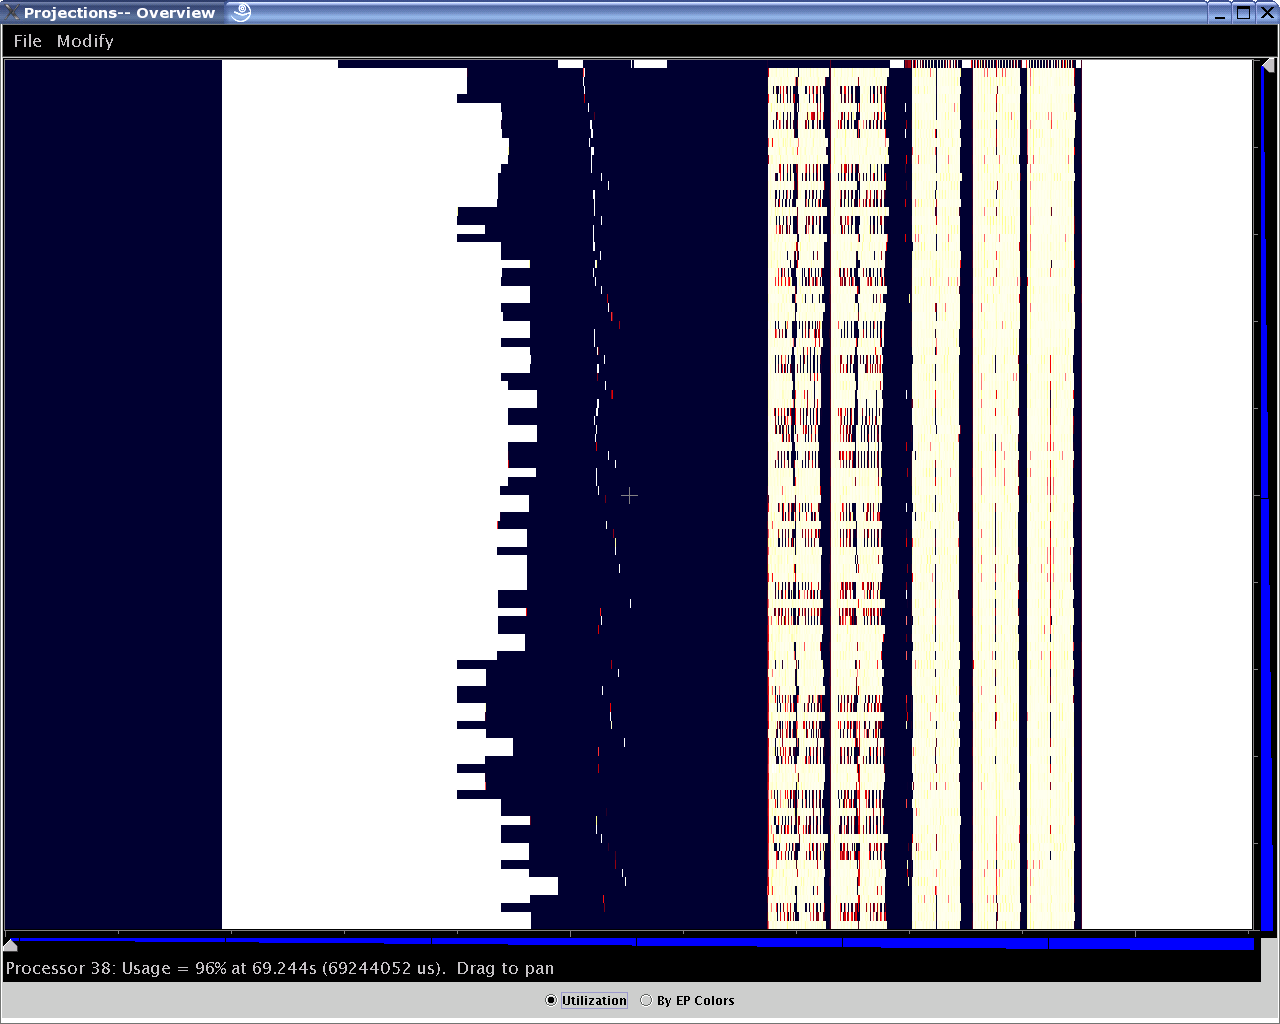
\includegraphics[width=4.0in]{fig/overview}
\caption{Overview}
\label{overview}
\end{figure}

This tool provides support for the following menu options:

\begin{itemize}
\item {\bf File} provides 1 option: {\it Close} closes the current tool.
\item {\bf Modify} provides 1 option: {\it Set Range} reloads the
dialog box and allows the user to specify new parameters for rendering
new overview information.
\end{itemize}

The view currently hard codes the number of intervals to 7,000
independent of the time-range desired.

Each processor has a row of colored bars in the display, different
colors indicating different utilization at that time (White
representing 100% utilization, shades of red representing other
utilization (100% < utilization < 0%) and the background color
representing 0% utilization. Moving a mouse over the graph will invoke
a display of the processor usage of the specific processor at the
specific time in the status bar below the graph. Vertical and
horizontal zoom is enabled by two zooming bars to the right and lower
of the graph. Panning is possible by clicking on any part of the
display and dragging the mouse.

The ``by EP colors'' radio button provides more detail by replacing
the utilization colors with the colors of the most significant entry
method execution time in that time-interval on that processor
represented by the cells. Be warned that this particular view is very
likely a major visualization resource hog.

The general Overview tool has no known resource usage issues and may
be used to load data for any time/processor range.

\subsubsection{Animations}

This window (see figure \ref{animation}) animates the processor usage
over a specified range of time and a specified interval size.

The dialog box to load animation information is exactly the same as
that of the Graph tool (see section \ref{sec::graph view}).

\begin{figure}[htb]
\center
%\epsfig{figure=fig/animation.eps,height=3in}
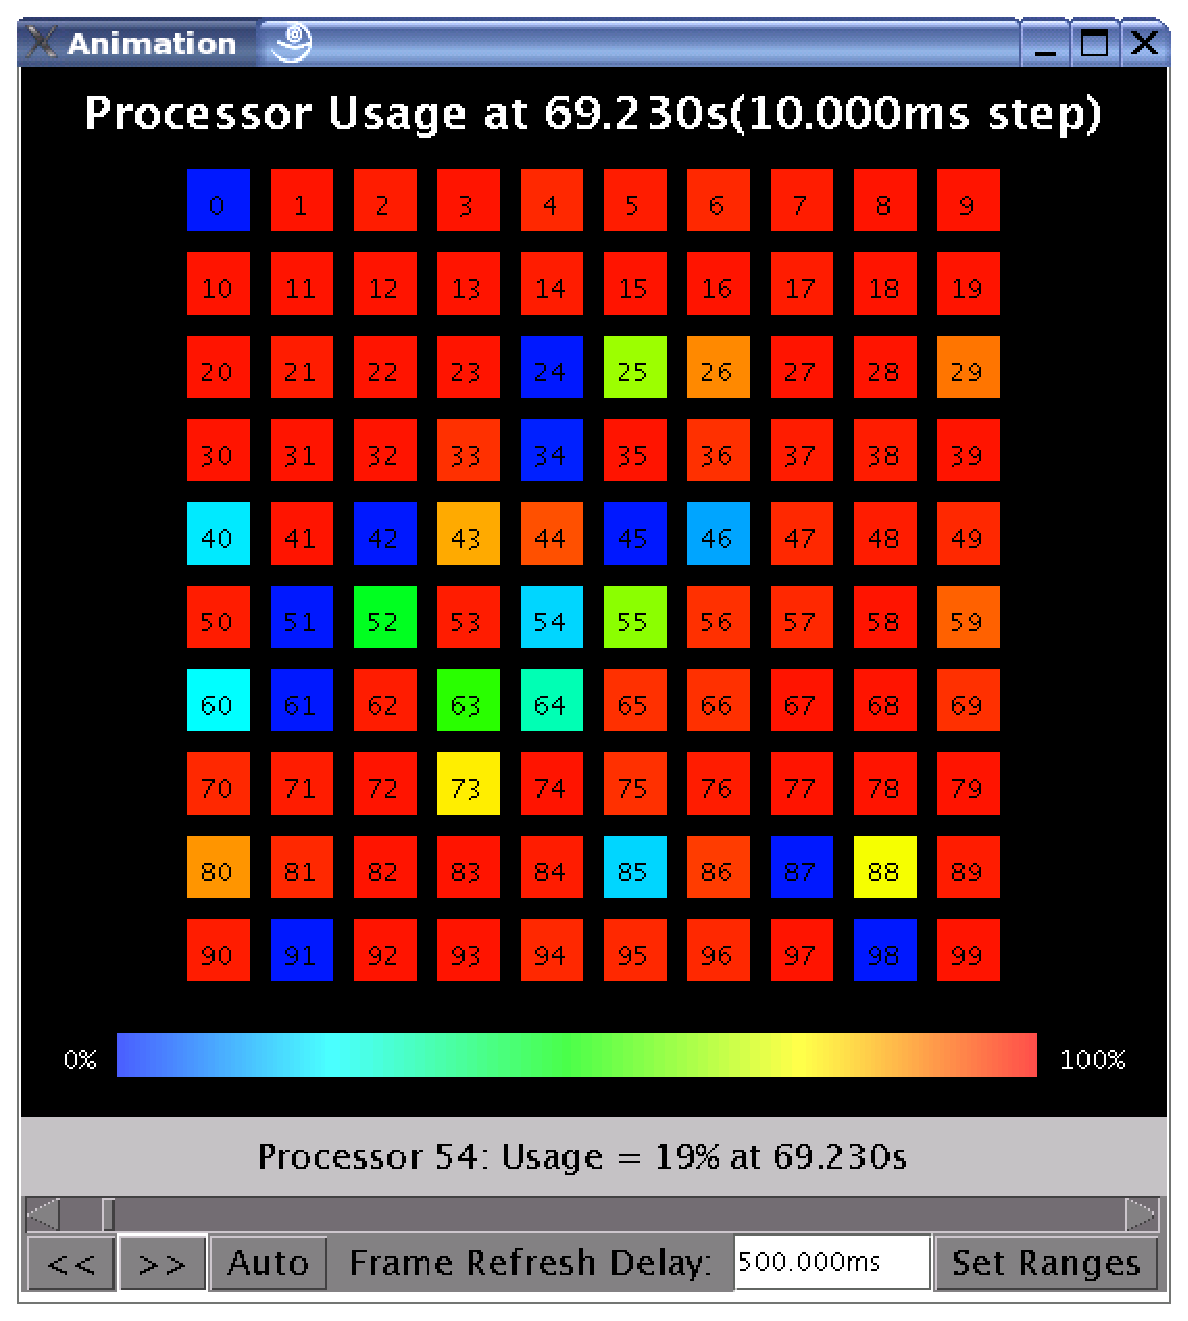
\includegraphics[width=2.5in]{fig/animation}
\caption{Animation View}
\label{animation}
\end{figure}

A color temperature bar serves as a legend for displaying different
processor utilizations as the animation progresses. Each time interval
will have its data rendered as a frame. A frame displays in text on
the top of the display the currently represented execution time of the
application and what the size of an interval is.

Each selected processor is laid out in a 2-D plot as close to a square
as possible. The view employs a color temperature ranging from blue
(cool - low utilization) to bright red (hot - high utilization) to
represent utilization.

You may manually update the frames by using the ``$<<$'' or ``$>>$''
buttons to visualize the preceding or next frames respectively. The
``Auto'' button toggles automatic animation given the desired refresh
rate.

The ``Frame Refresh Delay'' field allows you to select the real time
delay between frames. It is a time-based field (see section
\ref{sec::misc} for special features in using time-based
fields).

The ``Set Ranges'' button allows you to set new parameters for this
view via the dialog box.

This view has no known performance issues.

\subsubsection{Time Profile Graph}

The Time Profile view (see figure \ref{time profile}) is a
visualization of the amount of time contributed by each entry method
summed across all processors and displayed by user-adjustable time
intervals.

Time Profile's dialog box is exactly the same as that of the Graph
tool (see section \ref{sec::graph view}).

\begin{figure}[htb]
\center
%\epsfig{figure=fig/timeprofile.eps,height=4in}
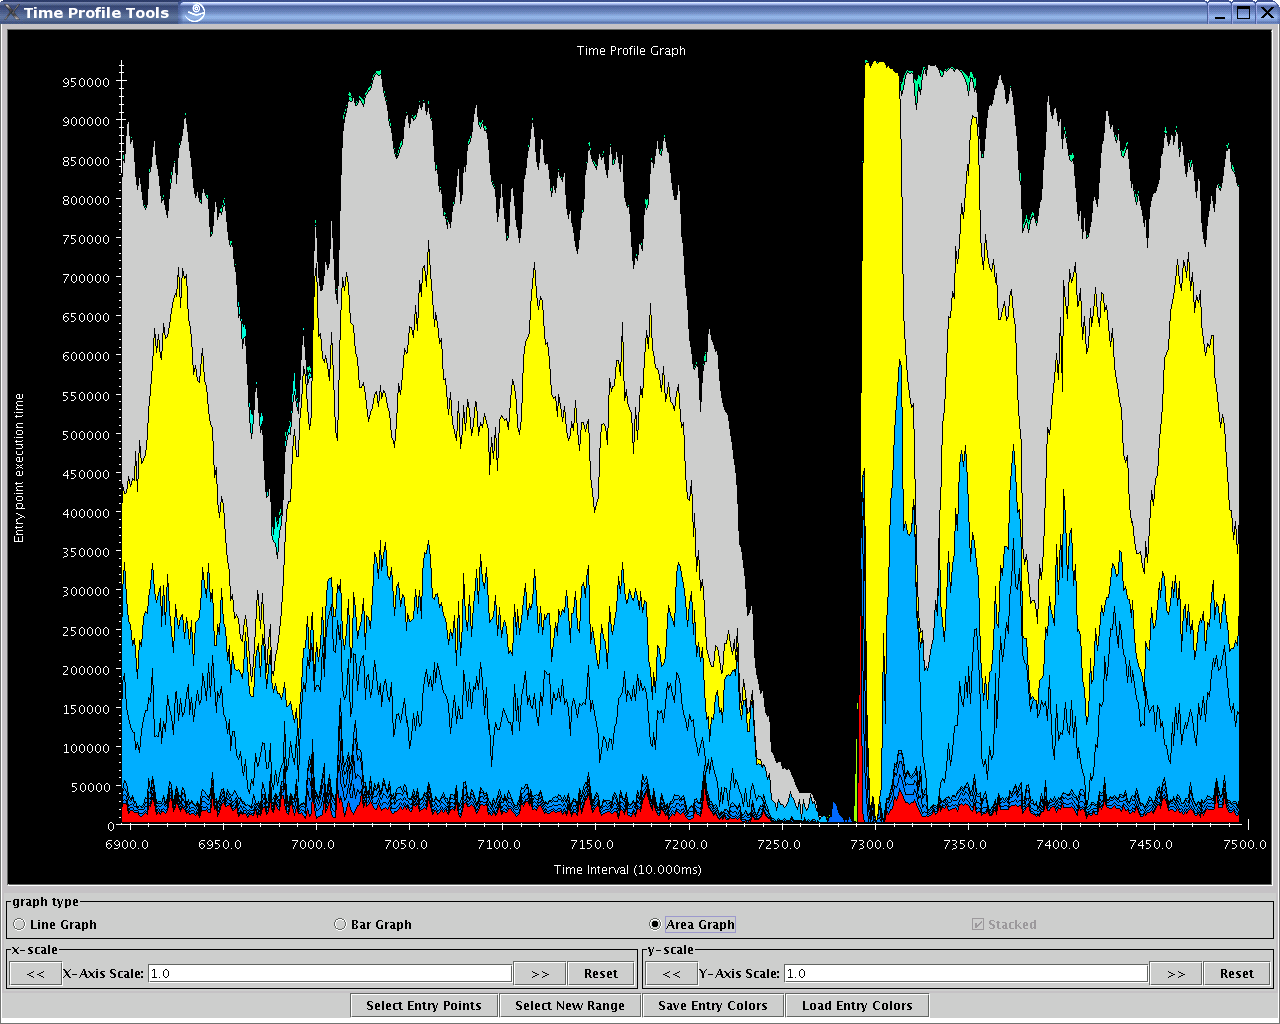
\includegraphics[width=4.0in]{fig/timeprofile}
\caption{Time Profile Graph View}
\label{time profile}
\end{figure}

Standard graph features can be employed for the main display of this
view (see section \ref{sec::misc}).

Under the tool options, one may:

\begin{itemize}
\item[-] Filter the set of entry methods to be displayed on the graph via
the ``Select Entry Points'' button. One may also modify the color set used
for the entry methods via this option.
\item[-] use the ``Select New Range'' button to reload the dialog box
for the tool and set new parameters for visualization (eg. different
time range, different set of processors or different interval sizes).
\item[-] store the current set of entry method colors to disk (to the
same directory where the trace logs are stored). This is done via the
``Save Entry Colors'' button.
\item[-] load the stored set of entry method colors (if it exists)
from disk (from the same directory where the trace logs are
stored). This is done via the ``Load Entry Colors'' button.
\end{itemize}

This tool's performance is tied to the number of intervals desired by
the user. We recommend that the user stick to visualizing 1,000
intervals or less.



\subsubsection{NoiseMiner View}

The NoiseMiner view (see figure \ref{time profile}) displays statistics about abnormally long entry methods. Its purpose is to detect symptoms consistent with \textit{Operating System Interference} or \textit{Compuatational Noise}. The abnormal events are filtered and clustered across multiple dimensions to produce a concise summary. The view displays both the duration of the events as well as the periodicity at which they occur. Its dialog box is exactly the same as that of the Graph tool (see section \ref{sec::graph view}).

The tool uses stream mining techniques to produce its results by making only one pass through the input data while using a limited amount of memory. This allows NoiseMiner to be very fast and scalable. 

\begin{figure}[htb]
\center
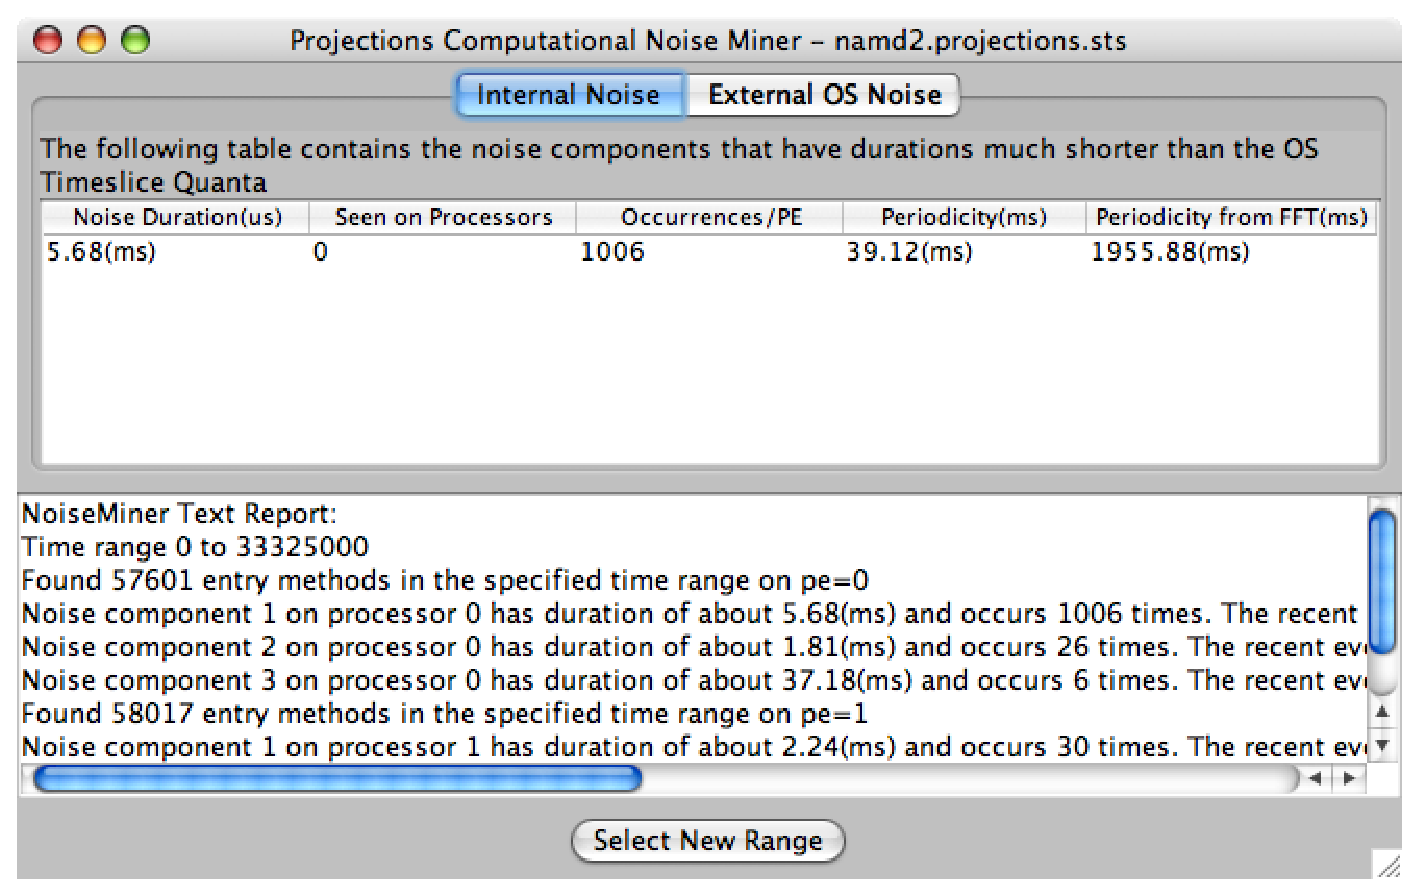
\includegraphics[width=4.0in]{fig/noiseminer}
\caption{NoiseMiner View displaying one \textit{Internal Noise} component of duration 5.68(ms) that occurred 1006 times during the run. This shows that there is likely some OS interference or Computational Noise problem occurring during the run. In this case, a faulty MPI implementation took an extra 5 ms to complete various calls which should have taken less than 0.1 ms.}
\label{noiseminer}
\end{figure}

NoiseMiner works by storing histograms of each entry method's duration. The histogram bins contain a window of recent occurrences as well as an average duration and count. After data stream has been parsed into the histogram bins, the histogram bins are clustered to determine the ``normal'' entry method duration. The histograms are then normalized by the ``normal'' duration so that they represent the abnormally stretched amounts for the entry methods. Then the histogram bins are clustered by duration and across processors. Any clusters that do not contribute much to the overall runtime are dropped. Finally each cluster is reported as shown in figure \ref{noiseminer}. The resulting clusters are displayed in one of two tabs: the \textit{Internal Noise} tab will list any events width periodicity significantly shorter than the OS time quantum which is currently hard-coded to 100ms while the \textit{External Noise} tab will list any events width periodicity close to or longer than the OS time quanta. A slightly more detailed text report is also provided in the bottom pane of the window for user's wishing to record the information for future reference.


\subsubsection{Miscellaneous features}
\label{sec::misc}

\begin{itemize}
\item[1)] 
{\bf Standard Graph Display}: A standard graph display (an
example of which can be found with the Main Summary Graph - figure
\ref{mainwindow}) has the following features:

\begin{itemize}
\item[-] {\bf Graph types} can be selected between ``Line Graph'' which
connects each data point with a colored line representing the
appropriate data entry. This information may be ``stacked'' or
``unstacked'' (controlled by the checkbox to the right). A ``stacked''
graph places one data point set (Y values) on top of another. An
``unstacked'' graph simply uses the data point's Y value to directly
determine the point's position; ``Bar Graph'' (the default) which
draws a colored bar for each data entry and the value of the data
point determines its height or starting position (depending on whether
the bar graph is ``stacked'' or ``unstacked''). A ``Bar Graph''
displayed in ``unstacked'' mode draws its bars in a tallest to
shortest order so that the large Y values do not cover over the small
Y values; ``Area Graph'' is similar to a ``Line Graph'' except that the
area under the lines for a particular Y data point set is also colored
by the data's appropriate color. ``Area Graph''s are always stacked.
\item[-] {\bf x-scale} allows the user to scale the X-Axis. This can be
done by directly entering a scaling factor in the text field (simple
numeric field - see below) or by using the ``$<<$'' or ``$>>$'' buttons
to increase or decrease the scale by 0.25 each time. The ``Reset'' button
changes the scale factor back to 1.0. A scrollbar automatically appears
if the scale factor causes the canvas to be larger than the window.
\item {\bf y-scale} allows the user to scale the Y-Axis. This functions 
similarly to the {\bf x-scale} feature where the buttons and fields are
concerned.
\end{itemize}

\item[2)]
{\bf Standard Dialog Features}

\begin{figure}[htb]
\center
%\epsfig{figure=fig/standard_dialog.eps,height=4in}
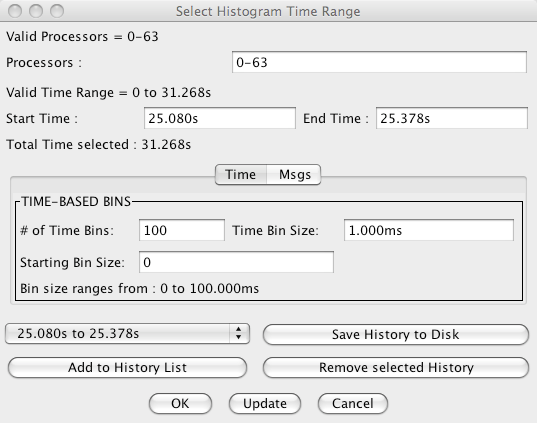
\includegraphics[width=2.5in]{fig/standard_dialog}
\caption{An example Dialog with standard fields}
\label{standard dialog}
\end{figure}

Figure \ref{standard dialog} shows a sample dialog box with standard
features. The following are standard features that can be employed in
such a dialog box:

\begin{itemize}
\item[-] {\bf Moving from field to field} via the tab key causes the
dialog box update the last field input by the user. It also performs a
consistency check. Whenever it finds an inconsistency, it will move
mouse focus onto the offending field, disabling the ``OK'' button so
as to force the user to fix the inconsistency. Examples of
inconsistency includes: input that violates a field's format; input
whose value violates constraints (eg. start time larger than end
time); or out-of-range stand-alone values.
\item[-] {\bf Available buttons} include ``OK'' which confirms the
user's choice of parameters. This button is only activated if the
dialog box considers the parameters' input to be
consistent. ``Update'' causes the dialog box to update the last field
input by the user and perform a consistency check. This is similar in
behavior to the user tabbing between fields. ``Cancel'' closes the
dialog box without modifying any parameters if the tool has already
been loaded or aborts the tool's load attempt otherwise.
\item[-] {\bf Parameter History} allows the user to quickly access
information for all tools for a set of frequently needed time
periods. An example of such a use is the desire by the analyst to view
a particular phase or timestep of a computation without having to
memorize or write on a piece of paper when exactly the phase or
timestep occurred.

It consists of a pull-down text box and 2 buttons. ``Add to History
List'' adds the current time range to the pull-down list to the left
of the button. The dialog box maintains up to 5 entries, replacing
older entries with newer ones. ``Save History to Disk'' stores current
history information to the file ``ranges.hst'' in the same directory
where your logs are stored. Note that you will need write access to
that directory to successfully store history information. A more
flexible scheme is currently being developed and will be released in a
later version of \projections{}. Clicking on the pull-down list allows
the user to select one out of up to 5 possible time ranges. You can do
so by moving the mouse up or down the list. Clicking on any one item
changes the start and end times on the dialog box.
\end{itemize}

\item[3)]
{\bf Data Fields}

Throughout \projections{} tools and dialog boxes (see sample figure
\ref{standard dialog}), data entry fields are provided. Unless
otherwise specified, these can be of the following standard field with
some format requirements:

\begin{itemize}
\item[-] {\bf Simple numeric fields}: An example can be found in
figure \ref{standard dialog} for ``Number of Bins:''. This field expects
a single number.
\item[-] {\bf Time-Based Field}: An example can be found in figure
\ref{standard dialog} for ``Start Time:''. This field expects a single
simple or floating point number followed by a time-scale modifier. The
following modifiers are supported: {\it none} - this is the default
and means the input number represents time in microseconds. A whole
number is expected; {\it The characters ``us''} - the input number
represents time in microseconds. A whole number is expected; {\it The
characters ``ms''} - the input number represents time in
milliseconds. This can be a whole number or floating point number; or
{\it The character ``s''} - the input number represents time in
seconds. This can be a whole number or floating point number.
\item[-] {\bf Processor-Based Field}: An example can be found in
figure \ref{standard dialog} for ``Processors:''. This field expects a
single whole number; a list of whole numbers; a range; or a mixed list
of whole numbers and ranges. Here are some examples which makes the
format clearer:

   eg: Want to see processors 1,3,5,7:  Enter {\tt 1,3,5,7}

   eg: Want to see processors 1,2,3,4:  Enter {\tt 1-4}

   eg: Want to see processors 1,2,3,7:  Enter {\tt 1-3,7}

   eg: Want to see processors 1,3,4,5,7,8: Enter {\tt 1,3-5,7-8}

Ranges also allow skip-factors. Here are some examples:

   eg: Want to see processors 3,6,9,12,15: Enter {\tt 3-15:3}

   eg: Want to see processors 1,3,6,9,11,14: Enter {\tt 1,3-9:3,11,14}

This feature is extremely flexible. It will normalize your input to a
canonical form, tolerating duplication of entries as well as
out-of-order entries (ie. {\tt 4,6,3} is the same as {\tt 3-4,6}).
\end{itemize}

\end{itemize}

\end{document}
